\chapter{Politique monétaire, forward guidance et stress systémique dans le cadre européen}
\mtcaddchapter
\minitoc

Dans un monde de plus en plus interconnecté où les crises se succèdent et ne se ressemblent pas, la stabilité économique et financière est l'enjeu le plus important pour assurer le bon fonctionnement du système global. Dans le cadre européen, cette stabilité repose en grande partie sur les actions de la BCE. Depuis sa création, la BCE a pour mission principale de garantir la stabilité des prix, un objectif central inscrit dans les traités européens. Cependant, la politique monétaire menée par la BCE a considérablement évolué au fil du temps, en réponse aux transformations économiques et aux crises successives qui ont mis sous pression le système financier européen. Historiquement, la politique monétaire reposait essentiellement sur des instruments conventionnels, tels que l’ajustement des taux directeurs et le contrôle de la liquidité bancaire à travers des opérations de refinancement. Toutefois, les chocs financiers majeurs de ces dernières décennies (notamment celle de 2008, des dettes souveraines en zone euro, plus récemment le COVID) ont profondément modifié le cadre d’action des banques centrales. Face à des situations inédites de taux d’intérêt proches de zéro et à des risques accrus d’instabilité financière, la BCE a dû innover et adopter de nouveaux outils pour assurer une transmission efficace de la politique monétaire. Parmi ces évolutions, la forward guidance s’est imposée comme un instrument central. Cette approche, qui consiste à fournir des indications sur l’orientation future de la politique monétaire, vise à influencer les anticipations des marchés et à renforcer l’impact des décisions monétaires sur l’économie réelle. En période de taux d’intérêt bas prolongés, où la marge de manœuvre des banques centrales se réduit, la forward guidance joue un rôle essentiel en stabilisant les anticipations et en facilitant la transmission de la politique monétaire. Cependant, son efficacité repose largement sur la crédibilité de la banque centrale et sur la cohérence des signaux envoyés aux investisseurs.

Parallèlement à ces évolutions monétaires, le stress systémique est devenu une préoccupation importante des décideurs économiques et des institutions financières. Le stress systémique désigne des tensions financières de grande ampleur qui, lorsqu’elles émergent, peuvent compromettre la stabilité du système financier dans son ensemble, il est signifié de réaction en chaîne ou d'effet domino. Ces tensions peuvent résulter de chocs exogènes, comme une crise bancaire, une forte volatilité des marchés ou encore une dégradation soudaine des conditions de financement. Si ces tensions ne sont pas contenues à temps, elles peuvent se propager rapidement via des effets de contagion et entraîner des répercussions négatives sur l’ensemble de l’économie. Les crises financières récentes ont illustré la vulnérabilité des marchés face à ces épisodes de stress prolongé. La crise des subprimes en 2008, qui a déclenché un effondrement mondial du système financier, et la crise des dettes souveraines en zone euro, qui a exacerbé les divergences entre les économies européennes, ont montré à quel point l’interconnexion des marchés pouvait amplifier la transmission des chocs. Ces événements ont poussé la BCE et d’autres institutions de régulation à renforcer leur surveillance des risques systémiques et à développer des outils de mesure plus sophistiqués. L’un des instruments clés dans ce domaine est l’Indicateur Composite de Stress Systémique (CISS), conçu pour évaluer les tensions financières en agrégeant plusieurs dimensions du stress de marché. Cet indicateur permet d’anticiper les périodes de vulnérabilité et de guider les actions des autorités monétaires afin de limiter les risques de contagion. Dans ce contexte, l’interaction entre politique monétaire, forward guidance et stress systémique constitue un sujet de recherche essentiel pour mieux comprendre comment la communication stratégique des banques centrales peut influencer la stabilité financière. Alors que la forward guidance est censée réduire l’incertitude et stabiliser les marchés en fournissant une trajectoire claire pour les taux d’intérêt, son impact sur le stress systémique reste une question ouverte. Dans certaines situations, une forward guidance mal calibrée ou perçue comme peu crédible peut au contraire accentuer la volatilité des marchés et amplifier les tensions financières.\\

L’objectif de ce chapitre est donc mettre en exergue et d’analyser comment la politique monétaire et la forward guidance interagissent avec le stress systémique en zone euro. Cette réflexion se structurera autour de trois grands axes. Les fondements de la politique monétaire en zone euro seront tout d’abord examinés. Cette section reviendra sur les objectifs et les instruments de la BCE, en mettant en lumière les transformations qu’a connues la politique monétaire européenne face aux crises successives. L’évolution des outils monétaires, de l’ère des instruments conventionnels aux politiques non conventionnelles, sera détaillée afin d’offrir une vision claire du cadre d’action actuel de la BCE. La forward guidance sera ensuite analysée comme un instrument clé de la politique monétaire moderne. Après une présentation de ses différentes formes cette section étudie les mécanismes par lesquels la forward guidance influence les anticipations et les marchés financiers. Les défis liés à sa mise en œuvre, notamment en matière de crédibilité et de cohérence des signaux monétaires, seront également abordés. La problématique du stress systémique et son interaction avec la forward guidance seront enfin approfondies. Cette dernière section mettra en évidence le rôle du CISS dans l’évaluation du stress financier et examinera comment la communication des banques centrales peut atténuer ou, au contraire, amplifier les tensions sur les marchés. L’importance de la coordination entre politique monétaire et régulation macroprudentielle sera également discutée, afin de comprendre comment ces deux leviers peuvent être articulés pour mieux gérer le risque systémique.

\section{Fondements de la politique monétaire}

Depuis sa création en 1998, la BCE a adopté une stratégie monétaire fondée sur une approche analytique et l’utilisation d’instruments adaptés aux évolutions du contexte économique et financier. Alors, l’objectif de cette section est d’analyser les fondements de la politique monétaire en zone euro, en mettant en évidence ses objectifs, ses stratégies et ses instruments. Cette analyse se déploie en trois temps. Tout d'abord, par une définition et objectifs de la politique monétaire avec une présentation des principes fondamentaux qui guident la politique monétaire en mettant l’accent sur le mandat de la BCE, son cadre institutionnel et les objectifs qu’elle poursuit. Aussi, il sera également présenté comment ces objectifs ont évolué dans le temps, notamment en réponse aux crises financières. Ensuite, il sera abordé les piliers de la stratégie monétaire de la BCE. Dans ce cadre, il sera mis en évidence l'analyse adopté par la BCE, en détaillant l’approche des deux piliers (analyse économique et monétaire) qui guide ses décisions. Cette section mettra en exergue les fondements théoriques et empiriques de cette stratégie, ainsi que les critiques qui lui sont adressées. Pour finir, l'évolution des instruments de la politique monétaire sera présenté historiquement ; l’ère de la stabilité initiale (1999-2008), marquée par l’utilisation d’outils conventionnels. La crise financière et la transformation de la politique monétaire (2008-2015), qui a vu l’introduction de mesures non conventionnelles comme les opérations de refinancement à long terme et les programmes d’achats d’actifs. La période post-crise et les défis de l’inflation basse (2015-2021), avec un recours accru à la forward guidance et aux politiques d’assouplissement quantitatif. La phase de normalisation et le choc inflationniste (2022-2024), qui marque un retour progressif à une politique plus restrictive face à une inflation élevée. Cela permettra de comprendre comment la BCE a dû adapter sa stratégie et ses outils en réponse aux défis économiques et financiers comtemporains, et comment la politique monétaire en zone euro est devenue un élément structurant de la stabilité macroéconomique et financière. Cette exploration permettra également de mieux comprendre l’importance croissante de la communication et des interactions entre la politique monétaire et les marchés financiers dans un contexte de plus en plus complexe et incertain.

\subsection{Définition et objectifs de la politique monétaire}

La politique monétaire repose sur un cadre d’analyse structuré permettant d’anticiper et de gérer les fluctuations économiques. Dans le cas de la BCE, cette approche s’articule autour de deux piliers complémentaires, combinant une évaluation des dynamiques économiques à court et moyen terme et une surveillance des évolutions monétaires susceptibles d’influencer l’inflation. Ces deux dimensions permettent d’assurer une prise de décision fondée sur une vision globale des risques pesant sur la stabilité des prix et l’activité économique.

\subsubsection{Définition}

La politique monétaire désigne l’ensemble des actions entreprises par une banque centrale pour réguler l’offre de monnaie et influencer les conditions financières dans une économie. Son objectif principal est d’assurer la stabilité des prix, c’est-à-dire maintenir l’inflation à un niveau compatible avec une croissance économique stable. La  BCE, en tant qu’autorité monétaire de la zone euro, a inscrit cet objectif dans son mandat, conformément à l’article 127 du Traité sur le Fonctionnement de l’Union Européenne (TFUE). La cible d’inflation est définie comme proche mais inférieure à 2\% à moyen terme (BCE, 2021).\\

Outre la stabilité des prix, la politique monétaire poursuit d’autres objectifs secondaires, notamment le soutien à la croissance économique et à l’emploi, conformément à l’approche flexible adoptée par la BCE depuis la crise financière de 2008 (Draghi, 2014). La stabilité financière, bien que non explicitement inscrite dans le mandat initial, est devenue une préoccupation majeure, comme en témoignent les mesures non conventionnelles mises en place après la crise des dettes souveraines en zone euro \citep{smets2003}.

\subsubsection{Les deux pilliers}

Depuis sa création en 1998, la BCE a adopté une stratégie monétaire fondée sur l’approche des "deux piliers", introduite par \citep{issing2001}. Cette approche permet d’évaluer les risques pesant sur la stabilité des prix en combinant une analyse économique et une analyse monétaire.\\

Le premier pilier, basé sur l’analyse économique, vise à évaluer les évolutions conjoncturelles susceptibles d’influencer l’inflation à court et moyen terme. Il repose sur l’examen de plusieurs indicateurs macroéconomiques, notamment la croissance du PIB, qui permet d’anticiper la dynamique économique globale, et le taux de chômage, qui donne des indications sur les pressions inflationnistes via le marché du travail \citep{blanchard1986}. Par ailleurs, l’évolution des prix des matières premières et des chocs d’offre externes est analysée pour détecter d’éventuels facteurs exogènes affectant l’inflation. Enfin, les conditions de financement, incluant les taux d’intérêt et l’accès au crédit bancaire, sont prises en compte pour évaluer la transmission de la politique monétaire et son effet sur l’activité économique \citep{smets2003}.\\

Le deuxième pilier, fondé sur l’analyse monétaire, repose sur l’idée que l’évolution de la masse monétaire joue un rôle clé dans la dynamique de l’inflation à long terme, en accord avec les théories monétaristes \citep{friedman1968}. Ainsi, la BCE surveille la croissance des agrégats monétaires, notamment M3, qui mesure la quantité de monnaie en circulation et son impact potentiel sur l’inflation. L’évolution du crédit bancaire est également étudiée, car elle reflète la transmission de la politique monétaire et son influence sur la consommation et l’investissement. En complément, la BCE analyse le comportement des institutions financières et les dynamiques des taux d’intérêt pour détecter d’éventuelles tensions financières susceptibles d’affecter l’économie réelle. Toutefois, certains économistes, comme \citep{gali2008}, ont critiqué la pertinence du second pilier, estimant que la relation entre masse monétaire et inflation est devenue plus floue dans un environnement de taux bas.\\

En réaction à des pilliers, une manière courante de modéliser la réaction de la politique monétaire aux variations macroéconomiques est la règle de Taylor, qui définit le taux d'intérêt nominal $i_t$ en fonction de l'inflation et de l'écart de production mais aussi de ses valeurs passées :

\begin{equation}
i_t = r^* + \pi_t + \sum_{k=0}^{K} \alpha_k (\pi_{t-k} - \pi^*) + \sum_{j=0}^{J} \beta_j (y_{t-j} - y^*)
\end{equation}

où  \( i_t \) est le taux directeur de la BCE à l’instant \( t \), \( r^* \) est le taux d’intérêt naturel, \( \pi_t \) est le taux d’inflation observé, \( \pi^* \) est la cible d’inflation de la BCE (proche mais inférieure à 2\%), \( y_t \) est le PIB réel, \( y^* \) est le PIB potentiel, \( \alpha \) et \( \beta \) sont les paramètres de réaction de la BCE à l’inflation et à l'écart de production. Cette équation traduit la manière dont la BCE ajuste ses taux en fonction de l’inflation et de l’écart de production. Une hausse de l’inflation au-delà de la cible ou une surchauffe économique incite la BCE à relever ses taux, tandis qu’une faible inflation ou un ralentissement économique justifie une politique monétaire plus accommodante.\\

Pour assurer la réalisation de ses objectifs, la politique monétaire s’appuie sur un ensemble d’instruments dont la nature et l’utilisation ont évolué au fil du temps. Si les outils traditionnels fondés sur la gestion des taux d’intérêt ont longtemps constitué la principale action des banques centrales, les bouleversements économiques et financiers des deux dernières décennies ont conduit à un élargissement et à une redéfinition de ces instruments.

\subsection{Évolution des instruments de la politique monétaire européenne}

L’évolution de la politique monétaire européenne reflète les transformations majeures qu’a connues la BCE face aux crises et aux mutations économiques. D’abord, la période de stabilité initiale (1999-2008) est abordée, illustrant une gestion classique des taux d’intérêt et de la liquidité bancaire. Ensuite, l’impact de la crise financière de 2008 et l’introduction d’instruments non conventionnels sont examinés, marquant une rupture avec les pratiques antérieures. La période post-crise et la problématique de l’inflation basse (2015-2021) sont ensuite analysées, soulignant l’importance croissante du quantitative easing et de la forward guidance. Enfin, la normalisation monétaire entamée à partir de 2022 face au choc inflationniste est présentée, mettant en lumière les défis actuels de la BCE dans un environnement économique incertain.\\

\subsubsection{L'ère de la stabilité initiale (1999-2008)}

Lors de sa création en 1999, la BCE a adopté une approche conventionnelle de la politique monétaire, inspirée des principes établis par la Bundesbank allemande. Durant cette période, l’outil principal de la BCE reposait sur la gestion des taux directeurs, notamment le taux de refinancement principal, utilisé pour contrôler l’inflation et stabiliser la croissance économique.\\

Durant cette décennie, la politique monétaire de la BCE était relativement prévisible et suivait une logique cyclique : les taux d’intérêt étaient ajustés en fonction de l’évolution de l’inflation et de la croissance. Par exemple, après la récession de 2001-2002 consécutive à l’éclatement de la bulle technologique, la BCE a progressivement réduit ses taux pour soutenir l’activité économique, avant de les relever à partir de 2005 pour contrer les tensions inflationnistes \citep{angeloni2003}. L’ensemble des opérations de refinancement (MRO, LTRO) était également utilisé dans une logique d’ajustement régulier de la liquidité bancaire, sans nécessiter d’intervention massive.

\newpage

Cependant, malgré cette stabilité apparente, des fragilités structurelles se sont développées, notamment une forte expansion du crédit et une augmentation de la prise de risque sur les marchés financiers, accentuées par une intégration croissante des économies européennes au sein de la zone euro \citep{bernanke2001}. Ces déséquilibres allaient se matérialiser de manière brutale avec la crise financière de 2008, marquant la fin de cette période de relative sérénité monétaire.

\subsubsection{La crise financière et la transformation de la politique monétaire (2008-2015)}

L’effondrement de Lehman Brothers en septembre 2008 marque un tournant important pour la politique monétaire mondiale et oblige la BCE à revoir en profondeur ses instruments d’intervention \citep{reinhart2009}. Face à un effondrement du crédit interbancaire, la BCE réduit drastiquement son taux de refinancement, passant de 4,25\% en juillet 2008 à 1\% en mai 2009 (ECB, 2009). Cependant, la persistance des tensions financières et la fragmentation du marché obligent l’institution à adopter des instruments non conventionnels, marquant une rupture avec son cadre initial et les traités européens signés à l'origine.\\

La BCE introduit ainsi les opérations de refinancement à long terme (LTROs), accordant des prêts massifs aux banques pour stabiliser le système financier \citep{coeuré2013}. Ces mesures visent à restaurer la transmission de la politique monétaire en assurant aux banques une liquidité suffisante pour financer l’économie réelle. Cependant, la crise des dettes souveraines de la zone euro (2010-2012) expose les limites des outils traditionnels : les écarts de taux entre les obligations d’État des différents pays de la zone euro s’élargissent dangereusement, menaçant l’intégrité même de l’union monétaire \citep{degrauwe2012}.\\

Face à cette crise existentielle, la BCE innove avec l’annonce du programme "Outright Monetary Transactions" (OMT) en 2012, qui permet d’acheter des obligations souveraines sous conditions. Mais c’est surtout le discours de Mario Draghi en juillet 2012, affirmant que la BCE fera "tout ce qu’il faudra" pour préserver l’euro, qui marque un tournant décisif (Draghi, 2012). Cette déclaration stabilise les marchés, illustrant l’importance croissante de la communication stratégique comme instrument de politique monétaire.

\subsubsection{La période post-crise et le défi de l’inflation basse (2015-2021)}

Après la crise des dettes souveraines, la zone euro entre dans une phase prolongée de faible inflation, voire de risque de déflation. La reprise économique reste fragile, et les anticipations d’inflation sont mal ancrées \citep{blanchard2015}. Confrontée à cette situation, la BCE adopte un arsenal monétaire encore plus expansif, mettant en place des mesures inédites dans l’histoire de la politique monétaire européenne.\\

L’instrument clé de cette période est le programme d’achats d’actifs (Quantitative Easing, QE) lancé en mars 2015 sous le nom de Public Sector Purchase Programme (PSPP). Ce programme consiste à acheter massivement des obligations souveraines et privées afin de faire baisser les taux d’intérêt à long terme et stimuler l’investissement et la consommation \citep{gürkaynak2015}. En complément, la BCE approfondit sa forward guidance, en s’engageant à maintenir des taux bas "aussi longtemps que nécessaire" pour ancrer les anticipations inflationnistes \citep{woodford2012}.\\

Une autre innovation majeure est l’introduction des opérations ciblées de refinancement à long terme (TLTROs), qui incitent les banques à accorder plus de crédits aux entreprises et ménages en leur offrant des conditions avantageuses \citep{altavilla2019}. Malgré ces efforts, l’inflation reste structurellement inférieure à l’objectif, en raison de facteurs démographiques, technologiques et de faiblesse de la demande \citep{blanchard2019}.\\

Le choc de la pandémie de Covid-19 en 2020 pousse la BCE à aller encore plus loin avec le Programme d’Achat d’Urgence face à la Pandémie (PEPP), un QE flexible visant à éviter une fragmentation financière excessive et à stabiliser l’économie. Ces actions marquent l’apogée des instruments non conventionnels, avec une politique monétaire extrêmement accommodante pour soutenir la reprise.

\subsubsection{Le choc inflationniste et la normalisation de la politique monétaire (2022-2024)}

Après une décennie de politique ultra-accommodante, le contexte change brutalement en 2022 avec un choc inflationniste majeur. La sortie de la pandémie, les perturbations des chaînes d’approvisionnement et la flambée des prix de l’énergie, exacerbée par la guerre en Ukraine, propulsent l’inflation bien au-delà de l’objectif de 2\%, atteignant 10,6\% en octobre 2022 (ECB, 2022).\\

Face à cette situation, la BCE amorce une normalisation rapide de sa politique monétaire sous la présidence de Christine Lagarde. En juillet 2022, elle met fin à son programme d’achats d’actifs, puis engage une série de hausses des taux directeurs, la première en plus de 10 ans. Le taux de refinancement, qui était à 0\% depuis 2016, est progressivement remonté pour atteindre 4,5\% en 2023 (ECB, 2023).\\

Cette phase de resserrement monétaire vise à freiner la demande et contenir l’inflation, au prix d’un ralentissement économique. Cependant, la BCE doit gérer un équilibre délicat entre lutte contre l’inflation et risque de récession, tout en évitant une fragmentation excessive des marchés obligataires de la zone euro. Pour y parvenir, elle introduit en 2022 le Transmission Protection Instrument (TPI), destiné à limiter les écarts de taux entre les États membres \citep{lane2023}.\\

En 2024, bien que l’inflation ait commencé à ralentir, les incertitudes restent fortes, et la BCE doit ajuster son action en fonction des perspectives économiques et financières. Cette période illustre le retour à une politique monétaire plus classique, mais avec un cadre profondément transformé par l’expérience des crises précédentes et l’usage d’instruments non conventionnels.\\

Parallèlement à ces ajustements, le rôle de la forward guidance et de la communication monétaire devient de plus en plus central. La BCE doit désormais convaincre les marchés que son action est efficace sans créer d’effets secondaires indésirables. L’incertitude économique oblige la banque centrale à ajuster ses discours et ses projections pour éviter des mouvements de panique ou d’anticipations excessives d’une récession \citep{nakamura2018}. Cette évolution illustre une tendance structurelle : la politique monétaire ne repose plus uniquement sur des décisions techniques, mais aussi sur la manière dont ces décisions sont perçues et anticipées par les acteurs économiques.\\

Ainsi, l’évolution de la politique monétaire européenne reflète les défis successifs auxquels la BCE a dû faire face, passant d’une gestion traditionnelle des taux d’intérêt à l’utilisation d’instruments non conventionnels en réponse aux crises financières et à la faiblesse persistante de l’inflation. Ainsi, il est essentiel de comprendre avant tout comment la politique monétaire se diffuse à travers les marchés.

\subsection{Transmission de la politique monétaire et interactions avec les marchés}

Avant d’examiner le rôle spécifique de la forward guidance dans le dispositif de transmission de la politique monétaire, il convient de revenir sur les fondements généraux de cette transmission. Celle-ci repose sur un ensemble de canaux identifiés dans la littérature, par lesquels les décisions de la banque centrale influencent l’économie réelle. Ces canaux, à la fois théoriques et empiriques, permettent d’évaluer l'efficacité des instruments monétaires selon les contextes macro-financiers.

\subsubsection{Les canaux de transmission de la politique monétaire : fondements théoriques et empiriques}

La transmission de la politique monétaire à l'économie réelle s'effectue à travers plusieurs canaux identifiés dans la littérature économique : le canal des taux d'intérêt, le canal du crédit bancaire, le canal du taux de change, et le canal des anticipations. Ces canaux sont largement étudiés dans les travaux de \citep{bernanke1995}, \citep{mishkin1996}, \citep{mishkin2001} et plus récemment par \citep{gertler2015} et \citep{boivin2010}. Ces mécanismes permettent d'évaluer l'efficacité des politiques monétaires menées par les banques centrales.\\

Le canal des taux d'intérêt repose sur l'idée que la politique monétaire influence directement les taux de marché à court terme, modifiant ainsi le coût du capital pour les entreprises et les ménages. Selon \citep{clarida2000}, les ajustements de taux directeurs sont censés influencer les décisions d'investissement et de consommation. Cependant, comme le souligne \citep{adrian2010}, en période de stress financier, la transmission peut être entravée par une augmentation des primes de risque.\\

Le canal du crédit bancaire souligne l’importance des institutions financières comme intermédiaires indispensables. Selon \citep{kashyap2000}, la contraction monétaire réduit la disponibilité du crédit en augmentant les contraintes de financement des banques, entraînant une diminution des prêts aux agents économiques. Ce phénomène est particulièrement exacerbé en période de crise financière, comme l'ont démontré \citep{ivashina2010} lors de la crise de 2008.

Le canal du taux de change est particulièrement pertinent dans les économies ouvertes. \citep{obstfeld2005} mettent en évidence que les variations des taux d'intérêt directeurs influencent fortement le taux de change et par conséquent les flux commerciaux et financiers. \citep{rey2015} montre que dans un contexte de forte mobilité internationale des capitaux, les marchés financiers internationaux amplifient ces effets, conduisant à une synchronisation accrue des cycles économiques à travers les pays.

Le canal des anticipations est fondé sur le concept de forward guidance, étudié notamment par \citep{woodford2012} et \citep{delnegro2015}. Ce canal met l'accent sur la capacité des banques centrales à influencer les anticipations des agents économiques à travers une communication crédible et transparente concernant l'orientation future des politiques monétaires.

\subsubsection{Interactions avec les marchés financiers : implications pour la politique monétaire}

Les marchés financiers jouent un rôle clé dans l'amplification ou l'atténuation des effets des politiques monétaires. Une littérature croissante, dont \citep{brunnermeier2014} et \citep{adrian2014}, souligne comment les conditions financières peuvent influencer la transmission monétaire en périodes normales comme en périodes de crise.

En période de tensions financières, comme observés durant la crise financière globale, les marchés deviennent particulièrement sensibles aux signaux des banques centrales, exacerbant les effets des annonces de politique monétaire. \citep{brunnermeier2009} montrent notamment comment les contraintes de liquidité sur les marchés financiers peuvent aggraver la transmission des chocs monétaires négatifs à l'économie réelle.

Par ailleurs, les travaux de \citep{gilchrist2012} et \citep{caldara2019} mettent en évidence l'importance des primes de risque financières comme indicateur clé influençant la transmission monétaire. En effet, des augmentations significatives des primes de risque peuvent neutraliser partiellement l'effet expansionniste d'une baisse des taux directeurs, notamment lorsque les marchés financiers anticipent une augmentation du risque de défaut.

Enfin, la communication et la crédibilité des banques centrales constituent des dimensions fondamentales pour gérer les interactions avec les marchés financiers. Selon \citep{hansen2016}, une communication claire réduit l'incertitude sur les marchés financiers et améliore ainsi la transmission monétaire. Inversement, une communication ambigüe peut aggraver la volatilité des marchés et compliquer l'atteinte des objectifs de politique monétaire.\\

L’analyse des fondements de la politique monétaire en zone euro a mis en évidence la transformation progressive du cadre d’intervention de la BCE face aux évolutions économiques et financières. Initialement fondée sur une gestion classique des taux directeurs, la politique monétaire européenne a dû s’adapter aux crises successives en développant des instruments non conventionnels, allant du quantitative easing aux opérations de refinancement à long terme. Cette évolution témoigne d’un passage d’une politique monétaire basée uniquement sur l’action des taux à une intégrant la communication stratégique et la gestion des anticipations. La transmission de la politique monétaire reste complexe, influencé par plusieurs canaux tels que les taux d’intérêt, le crédit bancaire, les marchés financiers et le taux de change. Ces mécanismes de transmission sont fortement dépendants du contexte économique et des réactions des agents financiers, rendant essentielle une communication claire et crédible de la banque centrale. L’interaction croissante entre la politique monétaire et les marchés financiers souligne l'importance d’un cadre cohérent de communication pour éviter des effets indésirables tels que la volatilité excessive des marchés ou une mauvaise interprétation des intentions de la banque centrale. Pour ce faire, il sera ensuite analysé en détail les mécanismes et enjeux de la forward guidance en étudiant ses différentes formes, son impact sur les anticipations des marchés et son rôle dans la transmission de la politique monétaire.


\section{La forward guidance : mécanismes et enjeux}

 Dans un environnement de taux bas et d’incertitude macroéconomique, la communication des banques centrales est devenue un outil essentiel de la politique monétaire. La forward guidance, qui consiste à donner des indications explicites sur l’orientation future des taux d’intérêt et d’autres instruments monétaires, joue un rôle central dans la formation des anticipations des marchés, des entreprises et des ménages \citep{hofmann2024ecb}. Cet article analyse le rôle de la forward guidance de la BCE dans la normalisation de sa politique monétaire. Il évalue également si la nouvelle approche de la BCE, basée sur des décisions "réunion par réunion" et dépendantes des données, peut renforcer la confiance du public et orienter les marchés financiers dans la direction souhaitée. Ce mécanisme est particulièrement important lorsque les taux atteignent leur borne inférieure effective, rendant les outils traditionnels de la politique monétaire moins efficaces. Il sera alors examiné les mécanismes sous-jacents de la forward guidance, ses différentes formes, ainsi que ses effets sur l’économie et les marchés financiers. Il est également porté une interrogation sur ses limites et les défis liés à son utilisation par les banques centrales. Pour ce faire il sera d'abord présenté une définition ainsi qu'une présentation des formes de la forward guidance tout en commençant précisément par définir la forward guidance et ses différentes formes. À travers l’exemple de la BCE, il sera analysé l’évolution de cette communication, depuis une guidance qualitative jusqu’à une approche conditionnelle basée sur des indicateurs économiques spécifiques. Ensuite, il sera mis en exergue les principaux canaux par lesquels la forward guidance influence l’économie. Il sera notamment étudié comment elle affecte les anticipations de taux futurs, les conditions financières des marchés d’actifs, l’ancrage des anticipations d’inflation, la transmission du crédit et son rôle en tant que signal sur l’état de l’économie. Enfin, il sera mis en lumière les défis liés à la forward guidance. Son efficacité dépend fortement du contexte macroéconomique et de la crédibilité des banques centrales. C'est pourquoi il sera discuté notamment des difficultés liées à sa mesure empirique, du rôle des anticipations des agents économiques et des risques d’incohérence temporelle qui peuvent nuire à sa crédibilité. 

\subsection{Définition et formes de la forward guidance}

La forward guidance s’est imposée comme un outil central de la politique monétaire moderne, particulièrement dans un environnement marqué par des taux d’intérêt bas et des incertitudes macroéconomiques accrues. Ce paragraphe examine d’abord la définition et les fondements théoriques de la forward guidance, en mettant en évidence son importance dans la transmission monétaire et son utilisation comme substitut aux outils traditionnels en période de contrainte sur les taux. Ensuite, elle explore les différentes formes qu’elle peut prendre, notamment dans le cas européen, où la BCE a progressivement adapté sa communication pour renforcer son efficacité. Cette transformation est passée d'une forward guidance qualitative à une approche basée sur des délais, puis conditionnelle plus précise.

\subsubsection{Définition}

La forward guidance est une stratégie de communication utilisée par les banques centrales pour influencer les anticipations des agents économiques concernant l’orientation future de la politique monétaire. Elle consiste à donner des indications explicites sur l’évolution prévue des taux d’intérêt directeurs ou d’autres instruments monétaires, dans le but de façonner les anticipations des marchés financiers, des entreprises et des ménages. Selon \citep{woodford2012}, la forward guidance permet aux banques centrales de moduler l’impact de leurs décisions présentes sur les anticipations de taux futurs, influençant ainsi les conditions financières et économiques avant même que des ajustements concrets de la politique monétaire ne soient mis en œuvre. L’objectif de la banque centrale est donc de minimiser l’écart de l’inflation à sa cible et l’écart de production, ce qui revient à minimiser la fonction de perte quadratique :

\begin{equation}
\ell_t = \frac{1}{2} \left[ (\pi_t - \pi^*)^2 + \lambda y_t^2 \right]
\end{equation}

\citep{blinder2017} ajoutent que la forward guidance peut être utilisée comme un substitut ou un complément aux outils monétaires traditionnels, notamment lorsque les taux d’intérêt atteignent leur borne inférieure effective (zero lower bound, ZLB) et ne peuvent plus être réduits davantage. \citep{blinder2000} définit une banque centrale comme crédible si « les gens croient qu’elle fera ce qu’elle dit », même si elle n’est soumise à aucune règle contraignante et qu’elle a un intérêt à ne pas respecter son engagement. D'autre part \citep{linta2024} explore la relation entre la forward guidance et la crédibilité des banques centrales. Elle souligne l'importance d'une communication transparente et cohérente pour assurer l'efficacité de la forward guidance en tant qu'outil de politique monétaire. En effet, la crise financière mondiale, la baisse tendancielle du taux d’intérêt réel d’équilibre, ainsi que la période prolongée de taux nominaux bloqués dans les principales économies avancées ont conduit à une réévaluation de la fréquence et de la gravité des épisodes contraints par la borne inférieure, ainsi que de l’efficacité des cadres de politique monétaire existants pour assurer la stabilité macroéconomique. Les banques centrales ont donc acquis une expérience significative dans l’utilisation d’instruments de politique monétaire non conventionnels, tels que la forward guidance sur l’orientation future des taux d’intérêt et les achats d’actifs à grande échelle. Ces instruments ont permis d’atténuer les effets négatifs de la borne inférieure sur l’activité économique et ont été essentiels pour préserver la stabilité des prix. 

\subsubsection{Les différentes formes de forward guidance : le cas européen}

La BCE a adopté la forward guidance à partir de 2013, dans un contexte de taux d’intérêt bas et de faible inflation après la crise financière mondiale et la crise des dettes souveraines en zone euro. Depuis, la BCE a utilisé différentes formes de forward guidance pour orienter les anticipations des marchés et influencer les conditions financières et économiques de la zone euro \citep{hofmann2024ecb}.\\

La forward guidance qualitative \citep{blinder2017}. La BCE a d’abord opté pour une forward guidance qualitative, en adoptant une communication vague et générale sur l’orientation future de sa politique monétaire. Cette approche s'est traduite par des déclarations telles que : \textit{« La politique monétaire restera accommodante aussi longtemps que nécessaire. »} Ce type de guidance a été introduit officiellement par la BCE en juillet 2013 sous la présidence de Mario Draghi, avec l’objectif de clarifier l’orientation de la politique monétaire après une longue période d’incertitude. À cette époque, la BCE souhaitait rassurer les marchés sur la pérennité de ses mesures de soutien face aux tensions économiques persistantes en zone euro. Toutefois, ce type de forward guidance a montré ses limites, car les marchés financiers et les agents économiques avaient du mal à anticiper avec précision la durée et l’ampleur de la politique monétaire accommodante. L'absence d'indications précises a limité l’impact de cette communication sur les taux d’intérêt à long terme et sur l’inflation anticipée.\\

La forward guidance basée sur des délais \citep{blinder2017} : une communication plus engageante. Face à la persistance de l’inflation faible et aux attentes de marché mal ancrées, la BCE a progressivement renforcé sa forward guidance en adoptant une approche basée sur des délais (calendar-based forward guidance). Dans cette forme, la BCE fixe une période précise durant laquelle les taux resteront à un niveau bas. Par exemple, dans ses communications, la BCE a précisé : \textit{« Les taux d’intérêt resteront à leur niveau actuel ou à un niveau inférieur au moins jusqu’à l’été 2019. » (Mario Draghi, conférence de presse, 2018)}. Ce type de guidance a eu pour effet de renforcer la prévisibilité de la politique monétaire et de réduire la volatilité des anticipations des marchés financiers. Cependant, un inconvénient majeur de cette approche est qu’elle contraint la banque centrale : si les conditions économiques évoluent plus rapidement que prévu, elle peut se retrouver coincée par son propre engagement, risquant de perdre en crédibilité si elle doit modifier sa politique avant la fin de la période annoncée. Un exemple notable est celui de la BCE en 2021-2022, où une hausse imprévue de l’inflation a conduit à un resserrement monétaire plus rapide que prévu, remettant en question la forward guidance précédente qui indiquait un maintien prolongé des taux bas.\\

La forward guidance conditionnelle \citep{blinder2017} : un engagement dépendant des données économiques. Pour éviter les limites des deux approches précédentes, la BCE a progressivement évolué vers une forward guidance conditionnelle (state-dependent forward guidance), où ses décisions futures sont liées à des indicateurs économiques spécifiques. Par exemple, dans sa stratégie adoptée en juillet 2021, la BCE a précisé que ses taux d’intérêt resteront bas jusqu’à ce que l’inflation atteigne durablement son objectif :
\textit{« Nous nous attendons à ce que les taux directeurs restent à leurs niveaux actuels ou plus bas jusqu’à ce que nous voyions l’inflation atteindre 2\% bien avant la fin de notre horizon de projection et de manière durable. » (Christine Lagarde, 2021)}.\\

L’évolution de la forward guidance au sein de la BCE illustre la montée en puissance de la communication stratégique comme instrument de politique monétaire. Cependant, pour comprendre l’impact de la forward guidance il est indispensable d’analyser les mécanismes par lesquels ces signaux se diffusent dans l’économie réelle.

\subsection{Mécanismes de transmission}

La forward guidance influence l’économie à travers plusieurs canaux de transmission qui interagissent avec les marchés financiers et les décisions des agents économiques. Cette section examine les principaux mécanismes à travers lesquels la communication des banques centrales modifie les comportements des investisseurs, des entreprises et des ménages.

\subsubsection{Anticipations des taux futurs}

Le premier mécanisme passe par l’anticipation des taux d’intérêt futurs. En annonçant sa volonté de maintenir les taux à un niveau bas pour une période prolongée, la banque centrale réduit les taux d’intérêt à long terme, qui intègrent les attentes de taux futurs. Cela favorise une baisse des coûts d’emprunt pour les entreprises et les ménages, stimulant ainsi l’investissement et la consommation. Ce mécanisme est particulièrement important lorsque les taux directeurs sont contraints par la borne inférieure effective (effective lower bound), rendant impossible une réduction supplémentaire des taux nominaux à court terme.\\ 

L'étude de \citep{coenen2021macroeconomic} examine l'efficacité de trois instruments de politique économique dans un contexte de faibles taux d'intérêt : la forward guidance dépendante de l'état, les achats d'actifs à grande échelle et les stimulus budgétaires basés sur les dépenses publiques. En s'appuyant sur le Nouveau Modèle de la Zone Euro (NAWM II) développé par la Banque centrale européenne, les auteurs évaluent ces politiques dans un cadre où la borne inférieure effective sur les taux d'intérêt nominaux contraint l'action monétaire. Leurs résultats mettent en évidence que, sans intervention, cette contrainte peut provoquer d’importantes distorsions macroéconomiques, notamment en maintenant une inflation inférieure à l’objectif et en freinant la croissance économique. Cependant, lorsque la forward guidance est pleinement crédible, elle constitue l’outil le plus efficace pour contrer ces effets négatifs, permettant ainsi de compenser largement les déséquilibres macroéconomiques. Toutefois, si cette forward guidance est perçue comme imparfaitement crédible, une combinaison d’instruments, incluant les achats d’actifs à grande échelle et les mesures de relance budgétaire, peut s’avérer presque aussi efficace. En particulier, les achats d’actifs renforcent la crédibilité de la forward guidance par un effet de signalisation, incitant ainsi les agents économiques à ajuster leurs anticipations de manière plus cohérente avec les objectifs de la banque centrale. Enfin, dans un scénario où le taux d’intérêt réel d’équilibre demeure proche de zéro à long terme, les auteurs soulignent la nécessité d’une approche combinée, mobilisant simultanément ces trois instruments pour réduire durablement les distorsions macroéconomiques. Ces conclusions mettent en exergue l’importance de la crédibilité des banques centrales et la nécessité d’adopter une stratégie intégrée afin de préserver la stabilité macroéconomique dans un environnement de taux d’intérêt durablement bas.\\

D'autre part, \citep{andrade2019}, à travers le Survey of Professional Forecasters, mettent en évidence l'existence d'un type de prévisionniste pessimiste qui, pendant la période de forward guidance, fait confiance à la Réserve fédérale (Fed) pour maintenir les taux d'intérêt bas, mais s'attend simultanément à une faible activité macroéconomique. Ce prévisionniste interprète donc l’annonce comme un signal de détérioration des conditions économiques, ce qui reflète un manque de confiance dans la capacité de la Fed à atteindre ses objectifs.\\

Le taux d’intérêt à long terme \( i_t^{LT} \) est défini comme la moyenne des taux courts futurs attendus :

\begin{equation}
i_t^{LT} = \sum_{k=0}^{\infty} \theta_k \mathbb{E}_t [i_{t+k}]
\end{equation}

où \( \theta_k \) est un facteur de pondération décroissant avec l’horizon temporel \( k \). Si la forward guidance ancre les taux d'intérêt attendus à \( i_t^{FG} \), il est obtenu :

\begin{equation}
\mathbb{E}_t [i_{t+k}] = i_t^{FG} + \rho_k
\end{equation}

où \( \rho_k \) représente un choc exogène. Ainsi, la courbe des taux devient :

\begin{equation}
i_t^{LT} = i_t^{FG} + \sum_{k=0}^{\infty} \theta_k \rho_k
\end{equation}

La banque centrale suit une règle de Taylor anticipative :

\begin{equation}
i_t = r^* + \mathbb{E}_t [\pi_{t+1}] + \alpha (\mathbb{E}_t [\pi_{t+1}] - \pi^*) + \beta (\mathbb{E}_t [y_{t+1}] - y^*)
\end{equation}

Si la forward guidance est crédible, alors :

\begin{equation}
\mathbb{E}_t [i_{t+1}] = i_t^{FG}
\end{equation}

En substituant dans la règle de Taylor :

\begin{equation}
i_t^{FG} = r^* + \mathbb{E}_t [\pi_{t+1}] + \alpha (\mathbb{E}_t [\pi_{t+1}] - \pi^*) + \beta (\mathbb{E}_t [y_{t+1}] - y^*)
\end{equation}

Ce qui donne la condition d'équilibre pour fixer la forward guidance :

\begin{equation}
i_t^{FG} - r^* = \mathbb{E}_t [\pi_{t+1}] + \alpha (\mathbb{E}_t [\pi_{t+1}] - \pi^*) + \beta (\mathbb{E}_t [y_{t+1}] - y^*)
\end{equation}

Il est donc évident que la forward guidance influence directement les anticipations des taux futurs et se transmet à l'économie via la réduction de l’incertitude sur les taux futurs \( i_t^{LT} \).\\

Par exemple, lors de sa réunion du 4 juillet 2013, la BCE a introduit pour la première fois une forward guidance explicite en déclarant que : \textit{« Le Conseil des gouverneurs s’attend à ce que les taux d’intérêt directeurs restent à leur niveau actuel ou à un niveau inférieur pour une période prolongée »}. Cette annonce visait à ancrer les anticipations dans un contexte de faible inflation et de reprise fragile, sans modifier immédiatement les taux. De même, en mars 2016, la BCE a combiné des taux négatifs, un programme d’achats d’actifs (QE), et une guidance précisant que les taux resteraient \textit{« à leurs niveaux actuels, ou plus bas, bien au-delà de l’horizon des achats »}. Ces décisions peuvent être interprétées à travers le modèle précédent : la forward guidance fixe un taux anticipé $i_t^{FG}$, qui influence la courbe des taux $i_t^{LT}$ via la somme pondérée des anticipations futures. Cela permet de transmettre plus efficacement la politique monétaire à l’économie réelle, notamment via le crédit et l’investissement, en réduisant l’incertitude sur les taux futurs. En liant la FG à une règle de Taylor anticipative, on comprend que la BCE ajuste son signal en fonction de ses anticipations d’inflation et d’activité : un signal de taux bas traduit soit une stratégie accommodante pour stimuler l’économie, soit, comme le souligne \citep{andrade2019}, une lecture pessimiste par les agents sur l’état futur de la conjoncture, révélant les ambiguïtés d’interprétation de la communication stratégique.

\subsubsection{Canal des conditions financières des marchés d'actifs}

La forward guidance affecte également l'économie en influençant les prix des actifs financiers. Une annonce de politique monétaire accommodante peut entraîner une baisse des rendements obligataires et une hausse des cours boursiers, améliorant ainsi la richesse des ménages (effet richesse). En parallèle, la baisse des taux d'intérêt pousse les investisseurs à rechercher des actifs plus risqués, ce qui stimule les marchés financiers et facilite le financement des entreprises.\\

\citep{swanson2021}, analyse l'impact des politiques monétaires non conventionnelles de la Réserve fédérale, notamment la forward guidance et les achats d'actifs à grande échelle (LSAPs), sur les marchés financiers durant la période où les taux d'intérêt étaient proches de zéro. Cette politique a significativement influencé les taux des bons du Trésor à court terme, les rapprochant des effets observés avec le taux des fonds fédéraux en période normale. Les achats d'actifs ont eu un effet notable sur les taux des obligations à long terme, tant du Trésor que des entreprises, surpassant l'impact de la forward guidance et du taux des fonds fédéraux sur ces maturités. En somme, l'étude de Swanson démontre que la forward guidance et les achats d'actifs ont eu des effets substantiels et statistiquement significatifs sur les marchés financiers, comparables en ampleur à ceux du taux des fonds fédéraux avant la contrainte de la borne inférieure zéro. La forward guidance a été particulièrement efficace pour influencer les taux à court terme, tandis que les LSAPs ont eu un impact plus marqué sur les taux à long terme.\\

Alors en reprenant \citep{swanson2021}, s'il est considéré un actif financier dont le prix \( P_t \) est déterminé par l’actualisation des flux futurs \( D_{t+k} \) (dividendes, coupons) en fonction des taux d’intérêt attendus \( i_{t+k} \).

\begin{equation} 
P_t = \sum_{k=1}^{\infty} \frac{\mathbb{E}_t [D_{t+k}]}{(1 + \mathbb{E}_t [i_{t+k}])^k} 
\end{equation}

Lorsque la banque centrale annonce une politique monétaire accommodante via la forward guidance, elle influence \( \mathbb{E}_t [i_{t+k}] \) de la manière suivante :

\begin{equation}
\mathbb{E}_t [i_{t+k}] = i_t - \theta \cdot FG_t
\end{equation}

où \( FG_t \) est l’annonce de forward guidance à \( t \), \( \theta > 0 \) est le coefficient d’impact de la guidance sur les taux d’intérêt. Ainsi, une forward guidance plus accommodante (\( FG_t \) positif) réduit les taux futurs attendus, ce qui augmente le prix des actifs \( P_t \), stimulant ainsi l’investissement et la consommation via l’effet richesse.

\subsubsection{Ancrages des anticipations d'inflations}

En annonçant sa politique future, la banque centrale peut influencer les anticipations d'inflation des ménages et des entreprises. Une forward guidance crédible ancre les anticipations d'inflation au niveau cible, évitant ainsi une spirale déflationniste lorsque l'économie est en sous-performance. En anticipant une inflation future plus élevée, les entreprises augmentent leurs prix et les ménages accélèrent leurs décisions de consommation, stimulant ainsi l'activité économique. \citep{coenen2021macroeconomic} soulignent que l'efficacité de la forward guidance dépend fortement de la crédibilité de la banque centrale dans l’ancrage des anticipations.

\subsubsection{Canal du crédit et de la transmission bancaire}

En abaissant les taux d'intérêt attendus, la forward guidance affecte également les coûts de financement des banques et, par extension, l'offre de crédit à l'économie. Des taux bas incitent les banques à accorder plus de prêts, favorisant ainsi l'investissement des entreprises et la consommation des ménages. Toutefois, si la forward guidance dure trop longtemps, elle peut réduire la rentabilité des banques et les inciter à rationner le crédit, ce qui peut limiter ses effets stimulants. \citep{bernanke1995} décrivent comment la politique monétaire influence l'offre de crédit via le canal bancaire. L’offre de crédit par les banques peut être modélisée à travers une équation inspirée du modèle de prêt bancaire de \citep{bernanke1988credit}, reliant le volume de crédit \( L_t \) aux taux d’intérêt et à la rentabilité bancaire.

\begin{equation} L_t = \psi \left( \mathbb{E}_t [i_{t+k}] - r_d \right) - \kappa R_t 
\end{equation}

où \( L_t \) est l’offre de crédit bancaire à \( t \), \( \mathbb{E}_t [i_{t+k}] \) est le taux d’intérêt futur anticipé, \( r_d \) est le coût de financement des banques (dépôts et autres sources de financement), \( R_t \) représente la rentabilité bancaire (marge d’intérêt nette), \( \psi > 0 \) mesure la sensibilité de l’offre de crédit aux taux d’intérêt futurs, \( \kappa > 0 \) représente l’effet négatif de la baisse de rentabilité sur l’offre de prêts. Lorsque la forward guidance signale des taux bas prolongés, cela réduit \( \mathbb{E}_t [i_{t+k}] \), stimulant par la suite l’offre de crédit via la baisse des coûts d’emprunt des entreprises et des ménages. Puis, le processus réduit la rentabilité des banques en comprimant les marges d’intérêt, ce qui peut, à terme, limiter l’offre de prêts (\( R_t \) diminue, ce qui réduit \( L_t \) si la forward guidance est prolongée).

\subsubsection{ Le canal des effets de signalisation et de la crédibilité}

Enfin, la forward guidance agit via un effet de signalisation : elle renseigne les agents économiques non seulement sur l'orientation future des taux, mais aussi sur l’évaluation que la banque centrale fait de la conjoncture économique. Si la forward guidance est perçue comme un engagement fort, elle peut renforcer la confiance des marchés et stabiliser les anticipations. En revanche, une forward guidance ambiguë ou non crédible peut provoquer de l’incertitude et diminuer son efficacité.\\

\citep{nakamura2018}, examinent comment les annonces de politique monétaire de la Réserve fédérale américaine influencent les anticipations des agents économiques concernant l'état futur de l'économie. Les auteurs constatent qu'une augmentation des taux d'intérêt par la Fed entraîne non seulement une hausse des taux nominaux et réels à long terme, mais aussi une augmentation des prévisions de croissance économique. Ce résultat est contraire aux prédictions des modèles standards, qui anticipent une baisse de la croissance suite à un resserrement monétaire. Cette observation suggère que les décisions de politique monétaire communiquent aux marchés des informations sur les perspectives économiques. Par exemple, une hausse des taux peut être interprétée comme un signal de confiance de la Fed dans la solidité de l'économie, incitant les agents à revoir à la hausse leurs anticipations de croissance. La forward guidance, en plus de signaler la trajectoire future des taux, fournit des indications sur l'évaluation par la banque centrale de la conjoncture économique. Ainsi, une annonce de maintien des taux bas pourrait être perçue comme une anticipation de conditions économiques moins favorables, influençant les anticipations des agents en conséquence. C'est pourquoi un vecteur de crédibilité peut être ajouté dans la modélisation classique. L’inflation future est supposée suivre une courbe de Phillips anticipative :

\begin{equation}
\mathbb{E}_t [\pi_{t+1}] = \gamma \pi_t + \delta y_t + \varepsilon_t
\end{equation}

\( \gamma \) persistance de l’inflation (entre 0 et 1), \( \delta > 0 \) : sensibilité de l’inflation à l’output gap, \( \varepsilon_t \sim \mathcal{N}(0, \sigma^2) \) : choc de demande aléatoire.  L’écart de production suit une dynamique sous forme d’équation d’IS modifiée :

\begin{equation}
y_t = -\phi (i_t - \mathbb{E}_t [\pi_{t+1}] - r^*) + \eta_t
\end{equation}

avec \( \phi > 0 \) : sensibilité de la demande aux taux d’intérêt et \( \eta_t \sim \mathcal{N}(0, \sigma_\eta^2) \) un choc d’offre aléatoire. Il est ensuite possible de remplacer \( \mathbb{E}_t [\pi_{t+1}] \) dans l’équation classique de Taylor\footnote{Sous l'espérance conditionnelle $\mathbb{E}_t$, le choc $\varepsilon_t$ est pris en compte, tandis que $\eta_t$, réalisé à l'instant $t$, n'intervient pas dans l'anticipation de $y_{t+1}$.} :

\begin{equation}
i_t = r^* + \mathbb{E}_t [\pi_{t+1}] + \alpha (\mathbb{E}_t [\pi_{t+1}] - \pi^*) + \beta (\mathbb{E}_t [y_{t+1}] - y^*)
\end{equation}

En substituant la courbe de Phillips :

\begin{equation}
i_t = r^* + (\gamma \pi_t + \delta y_t) + \alpha (\gamma \pi_t + \delta y_t - \pi^*) + \beta (\mathbb{E}_t [y_{t+1}] - y^*)  
\end{equation}

Soit en déplaçant les termes :

\begin{equation}
i_t - r^* = (1 + \alpha) \gamma \pi_t + (1 + \alpha) \delta y_t - \alpha \pi^* + \beta (\mathbb{E}_t [y_{t+1}] - y^*)
\end{equation}

Or, l’output gap suit :

\begin{equation}
y_t = -\phi (i_t - \mathbb{E}_t [\pi_{t+1}] - r^*) + \eta_t
\end{equation}

En anticipant à \( t+1 \) :

\begin{equation}
\mathbb{E}_t [y_{t+1}] = -\phi (\mathbb{E}_t [i_{t+1}] - \mathbb{E}_t [\pi_{t+2}] - r^*)
\end{equation}

Par substitution dans l’équation de Taylor, il est obtenu une relation récursive :

\begin{equation}
i_t = r^* + (1+\alpha) \gamma \pi_t + (1+\alpha) \delta y_t - \alpha \pi^* - \beta \phi (\mathbb{E}_t [i_{t+1}] - \mathbb{E}_t [\pi_{t+2}] - r^*)
\end{equation}

Ainsi, si la forward guidance est crédible, alors les agents forment leurs anticipations rationnellement soit que $\mathbb{E}_t [i_{t+1}] = i_t$, ce qui donne : 

\begin{equation}
i_t = r^* + (1+\alpha) \gamma \pi_t + (1+\alpha) \delta y_t - \alpha \pi^* - \beta \phi (i_t - \mathbb{E}_t [\pi_{t+2}] - r^*)  
\end{equation}

Cela signifie que la forward guidance permet de fixer les attentes et d’influencer directement l’inflation et l’output gap, ce qui renforce la transmission monétaire.
En revanche, si la credibilité est faible, alors $i_t$ devient instable et renforce le stress.\\

\citep{linta2024} décrit comment la crédibilité de la banque centrale, mesurée par le degré d'unanimité au sein de son comité de politique monétaire, influence l'efficacité de la forward guidance. En utilisant des données à haute fréquence dans le cadre institutionnel de la BCE, l'étude révèle que l'absence d'unanimité au sein du Conseil des gouverneurs incite les marchés financiers à douter de l'engagement de la BCE concernant ses promesses de forward guidance. Ainsi, malgré des annonces accommodantes, les marchés anticipent un possible resserrement de la politique monétaire, ce qui atténue l'impact escompté de la forward guidance. En revanche, une unanimité affichée ne semble pas renforcer significativement l'efficacité de cette communication.\\

L’analyse des mécanismes de transmission met en évidence la complexité et la richesse des canaux par lesquels la forward guidance influence l’économie réelle. Cependant, si cet outil présente des atouts certains, notamment en période de contrainte sur les taux d’intérêt, il comporte aussi de nombreuses limites.

\subsection{Avantages et limites}

La forward guidance est un outil puissant de la politique monétaire, mais son efficacité est sujette à plusieurs limites et défis. Ce paragraphe examine les principales difficultés liées à son utilisation, en mettant en évidence les contraintes empiriques et théoriques qui compliquent son évaluation et son efficacité.

\subsubsection{La forward guidance inobservable difficile à quantifier}

L’un des principaux défis de l’analyse de la forward guidance réside dans son caractère inobservable. Contrairement aux instruments traditionnels de la politique monétaire, tels que la variation des taux directeurs ou les achats d’actifs, la forward guidance repose uniquement sur des déclarations de la banque centrale, sans action immédiate et directement mesurable. Son efficacité dépend donc entièrement de la manière dont elle est perçue par les agents économiques, notamment les marchés financiers, les entreprises et les ménages.\\

L’un des principaux obstacles à l’évaluation empirique de la forward guidance est l’absence d’un indicateur directement observable permettant de mesurer la force de l’engagement de la banque centrale. En effet, si une banque centrale annonce son intention de maintenir les taux bas pendant une période prolongée, comment s’assurer que les agents économiques perçoivent cet engagement comme crédible et contraignant ?\\

Les études empiriques tentent de contourner ce problème en analysant les réactions des marchés financiers suite aux annonces de forward guidance. \citep{swanson2021} montre par exemple que la forward guidance a eu un impact significatif sur les taux d’intérêt à long terme, mais cet effet varie selon la crédibilité perçue de la banque centrale. \citep{campbell2012} soulignent également que les marchés peuvent réagir différemment selon l’interprétation qu’ils font des annonces de politique monétaire, rendant ainsi difficile une évaluation systématique de leur impact.

\subsubsection{Le rôle des anticipations et des modèles économiques}

Dans un cadre théorique, la forward guidance fonctionne en influençant les anticipations des agents économiques concernant l’évolution future des taux d’intérêt et de la politique monétaire. Or, ces anticipations sont elles-mêmes inobservables, obligeant les économistes à utiliser des modèles basés sur des simulations et des approximations statistiques. Par exemple, \citep{nakamura2018} montrent que la forward guidance transmet des informations non seulement sur l’orientation future des taux, mais aussi sur l’état futur de l’économie, ce qui complique encore davantage son identification empirique. \citep{delnegro2015} utilisent des modèles DSGE pour tenter de quantifier l’impact de la forward guidance sur l’inflation et la croissance, mais leurs résultats dépendent fortement des hypothèses sous-jacentes sur la formation des anticipations des agents.

\subsubsection{Une efficacité dépendante du contexte macroéconomique}

L’efficacité de la forward guidance varie selon le contexte macroéconomique et le niveau de crédibilité de la banque centrale. Par exemple, en période de taux bas contraints par la borne inférieure effective, la forward guidance peut jouer un rôle essentiel en influençant les taux à long terme \citep{eggertsson2003}. En revanche, si les marchés doutent de la capacité de la banque centrale à maintenir ses engagements (par exemple en raison de pressions inflationnistes imprévues), son efficacité est réduite. Une étude de \citep{coenen2021macroeconomic} montre ainsi que lorsque la forward guidance est imparfaitement crédible, elle doit être complétée par d’autres instruments comme les achats d’actifs pour assurer un impact significatif sur l’économie. Cela fait échos à \citep{lucas1976}, la forward guidance repose sur l’anticipation rationnelle des agents : si les agents changent leur comportement en réponse à un changement de règle de politique monétaire, alors les effets estimés de cette politique ne sont plus valides une fois qu'elle est mise en œuvre.

\subsubsection{Risque d’incohérence temporelle et de perte de crédibilité}

Un autre problème réside dans le risque d’incohérence temporelle. La forward guidance implique que la banque centrale s’engage aujourd’hui à une politique future. Mais si, dans quelques années, les conditions économiques évoluent de manière imprévue, elle pourrait être tentée de ne pas respecter son engagement, ce qui nuirait à sa crédibilité.\\

\citep{blinder2000} souligne que la crédibilité d’une banque centrale repose sur la confiance des agents économiques : si ces derniers anticipent un revirement de politique avant la fin de la période annoncée, l’impact de la forward guidance est fortement réduit. \citep{kiley2018} montre également que lorsque les engagements de forward guidance sont perçus comme temporaires ou réversibles, leur effet sur les taux d’intérêt et l’activité économique est limité.\\

L'analyse de la forward guidance a montré son rôle central dans la politique monétaire moderne, en particulier lorsque les taux d'intérêt sont contraints par leur borne inférieure effective. En influençant directement les anticipations des agents économiques, elle permet d’agir sur les taux d'intérêt à long terme, les conditions financières et la stabilité macroéconomique. Son efficacité repose néanmoins sur plusieurs conditions, notamment la crédibilité de la banque centrale, la clarté des signaux envoyés aux marchés et l'adéquation entre les engagements pris et l'évolution des conditions économiques. Si la forward guidance a prouvé son utilité en tant qu’outil de stabilisation et de relance, elle présente aussi des limites et des risques, notamment en matière de crédibilité et de cohérence temporelle. Une guidance mal calibrée ou perçue comme réversible peut perdre son efficacité, voire générer de l’instabilité sur les marchés financiers. C’est pourquoi son utilisation doit être accompagnée d’une régulation macroprudentielle et d’autres instruments monétaires afin de minimiser les effets indésirables sur le système financier. Dans cette optique, il est nécessaire de s’intéresser à la notion de stress systémique en Europe, en analysant ses causes, ses mécanismes de propagation et ses conséquences pour la stabilité économique. Une attention particulière sera portée à l’indicateur composite de stress systémique (\textit{CISS}).

\section{Stress systémique dans le cadre européen}

La stabilité du système financier constitue une condition essentielle au bon fonctionnement des économies modernes, en particulier dans le cadre européen, où l’intégration des marchés financiers a été profondément développée. Cependant, cette interconnexion croissante entre les institutions financières, les marchés et les économies nationales a également accru le risque de propagation des crises. Ainsi, des épisodes de stress systémique peuvent émerger, compromettant non seulement la stabilité des marchés financiers, mais également celle de l’économie réelle. La compréhension des dynamiques du stress systémique en Europe revêt dès lors une importance capitale pour les décideurs économiques et les institutions financières, qui doivent être en mesure d’anticiper et d’atténuer les effets des crises financières. Le stress systémique peut être défini comme la matérialisation du risque systémique, c'est-à-dire l’émergence de tensions significatives au sein du système financier, susceptibles d’entraîner des effets en cascade affectant l’ensemble de l’économie. En période de forte incertitude, il est observé que des chocs localisés, initialement circonscrits à un segment du marché, se propagent rapidement à d’autres secteurs via différents canaux. Parmi ces canaux figurent notamment l’interconnexion des institutions financières, qui intensifie la transmission des risques, les réactions synchronisées des investisseurs, qui amplifient la volatilité des prix des actifs, ainsi que la dépendance des entreprises et des ménages au financement bancaire. Ces phénomènes ont été particulièrement mis en évidence lors de la crise financière mondiale de 2008 et de la crise des dettes souveraines en zone euro, deux épisodes qui ont révélé d’importantes vulnérabilités au sein du marché financier européen. Il est donc mené une analyse approfondie des mécanismes du stress systémique en Europe sera menée en plusieurs étapes. Tout d’abord, les bases théoriques seront posées afin de définir le risque systémique dans ses différentes dimensions. Une distinction sera établie entre les formes d’événements systémiques et leurs niveaux d’intensité, permettant ainsi d’identifier les mécanismes de propagation des crises financières. Ensuite, les manifestations du stress financier seront étudiées à travers l’observation des principaux symptômes affectant les marchés, tels que l’augmentation de la volatilité des actifs, l’élargissement des primes de risque ou encore la dégradation des conditions de liquidité. Une bonne mesure du stress systémique est ensuite présentée via l’indicateur composite de stress systémique (\textit{CISS}), qui constitue un outil essentiel pour mesurer et anticiper les tensions financières en Europe. Son évolution historique sera retracée, depuis les premiers indicateurs sectoriels jusqu’à son développement actuel, intégrant une approche globale prenant en compte les interdépendances entre marchés. Sa méthodologie de construction et son mode de calcul seront détaillés, en mettant en évidence la manière dont il permet de capter les dynamiques de propagation du stress financier. Une évaluation de son efficacité dans l’identification des périodes de vulnérabilité systémique sera également proposée, afin de mieux comprendre son rôle dans la surveillance et la prévention des crises financières. Enfin, une analyse des interconnexions entre les principaux segments du marché, actions, changes et interbancaire, sera menée. Il sera mis en lumière les mécanismes de contagion, qui jouent un rôle central dans l’amplification des crises financières et leur transmission à l’ensemble du système économique. Tout cela permettra de souligner les défis posés par le stress systémique dans le cadre européen et d’illustrer l’importance des outils de surveillance dans l’élaboration de politiques monétaires et macroprudentielles adaptées à la préservation de la stabilité financière.

\subsection{Définition et généralités sur le stress systémique}

Dans ce paragraphe il est défini le stress systémique comme la matérialisation du risque systémique, pouvant entraîner des crises financières majeures. Elle distingue les chocs idiosyncratiques, limités à une institution, des chocs systémiques qui affectent l’ensemble du système financier et l’économie réelle.

\subsubsection{Contexte théorique : risque systémique et stress financier}

Le risque systémique, dans un sens très général, n’est en aucun cas un phénomène limité à l’économie ou au système financier. L’illustration la plus naturelle de ce concept peut être trouvée dans le domaine de la santé et des maladies épidémiques. Dans les cas les plus graves (par exemple, la Grande Peste au Moyen Âge), une contamination généralisée par une maladie peut décimer une part significative de la population. C'est aussi un concept en macroéconomie monétaire qui désigne la probabilité qu’un choc ou une perturbation dans une partie du système financier entraîne des effets en chaîne susceptibles de compromettre son bon fonctionnement dans son ensemble. Ce type de risque se distingue des risques idiosyncratiques, qui sont spécifiques à une institution ou un marché particulier \textit{(microéconomique)} et qui, en l’absence d’interconnexion forte, ne se propagent pas nécessairement à l’ensemble du système. Le risque systémique est souvent associé aux crises financières, aux défaillances bancaires de grande ampleur, aux effondrements de marché et aux perturbations graves dans la transmission du crédit et des flux de capitaux. Lorsqu’il se matérialise, il peut affecter profondément l’économie réelle en réduisant la confiance des investisseurs, en freinant la consommation et l’investissement, et en aggravant les périodes de récession. In fine, ce risque peut entraîner la chute de l'ensemble du système. \\

Le stress systémique est interprété comme la part du risque systémique qui s’est déjà matérialisée. Le risque systémique, quant à lui, est défini comme le risque que l’instabilité financière devienne si généralisée qu’elle entrave le fonctionnement du système financier au point d’avoir un impact négatif significatif sur la croissance économique et le bien-être \citep{debandt2000systemic}, \citep{debandt2009systemic}.\\

Une distinction est faite entre deux perspectives du risque systémique.
La perspective horizontale, qui se focalise exclusivement sur le système financier. Elle analyse la manière dont les tensions émergent et se propagent au sein des marchés financiers, des institutions bancaires et des autres intermédiaires financiers. Cette approche met l’accent sur les dynamiques internes du système financier, telles que les effets de contagion, les liens interbancaires, la corrélation entre les classes d’actifs et les comportements procycliques des investisseurs.\\
Puis, une perspective verticale, qui prend en compte l’interaction bidirectionnelle entre le système financier et l’économie réelle. Elle étudie comment l’instabilité financière influence la consommation, l’investissement, l’emploi et la croissance économique, et, à l’inverse, comment les cycles économiques et les politiques économiques peuvent eux-mêmes générer ou atténuer les tensions macro-monétaires.\\

Donc, il faut comprendre que le risque systémique ne se limite pas aux banques et aux marchés financiers. Il concerne également les entreprises non financières, les ménages et les administrations publiques, qui sont tous affectés par les fluctuations des conditions de crédit, les variations des taux d’intérêt et la stabilité du système monétaire. Par exemple, une crise bancaire majeure peut entraîner un rationnement du crédit, limitant l’accès au financement pour les entreprises et freinant leur capacité à investir et à créer de l’emploi. De même, un effondrement du marché boursier peut réduire la richesse des ménages et affecter leur propension à consommer, ce qui produit un ralentissement économique et, potentiellement, une récession.

\subsubsection{Niveaux des évènements de risque systémique}

Il est défini un événement systémique au sens restreint comme un événement où la diffusion de "mauvaises nouvelles" concernant une institution financière, ou même sa faillite, ou encore l’effondrement d’un marché financier, entraîne, de manière séquentielle, des effets négatifs considérables sur une ou plusieurs autres institutions financières ou marchés, pouvant conduire à leur propre faillite ou effondrement. La zone ombrée dans la \autoref{fig:systemic_vents} englobe ces événements systémiques au sens restreint. L’élément essentiel de cette définition est l’"effet domino", où un choc initial limité (idiosyncratique) se propage d’une institution à l’autre ou d’un marché à l’autre.\\

Les événements systémiques au sens large, indiqués par des croix dans les zones ombrées et non ombrées de la \autoref{fig:systemic_vents}, englobent non seulement les événements mentionnés ci-dessus, mais aussi les effets négatifs simultanés sur un grand nombre d’institutions ou de marchés résultant de chocs graves et généralisés (systémiques). Il est évident que dans la mesure où ces impacts se produisent simultanément, cette catégorie inclut également les effets généralisés dus à la diffusion d’une nouvelle information (signaux).\\

Un événement systémique au sens restreint est qualifié de fort si les institutions affectées en second tour ou ultérieurement finissent effectivement par faire faillite à la suite du choc initial, bien qu’elles aient été fondamentalement solvables ex ante. De même, un événement est qualifié de fort si les marchés touchés dans les phases ultérieures s’effondrent, alors qu’ils ne l’auraient pas fait sans le choc initial. Ces instances particulièrement graves d’événements systémiques au sens restreint seront désignées sous un terme spécifique de contagion lorsque l'effet externe se traduit par une faillite ou un effondrement de marché. À l’inverse, si l’effet externe reste inférieur à une faillite ou à un crash, on parle d’événement systémique faible. De manière similaire, les événements systémiques liés à des chocs systémiques sont qualifiés de forts si une part significative des institutions financières ou des marchés affectés subissent effectivement des faillites ou des effondrements simultanés. Dans le cas contraire, ces événements sont qualifiés de faibles.

\begin{figure}
    \centering
    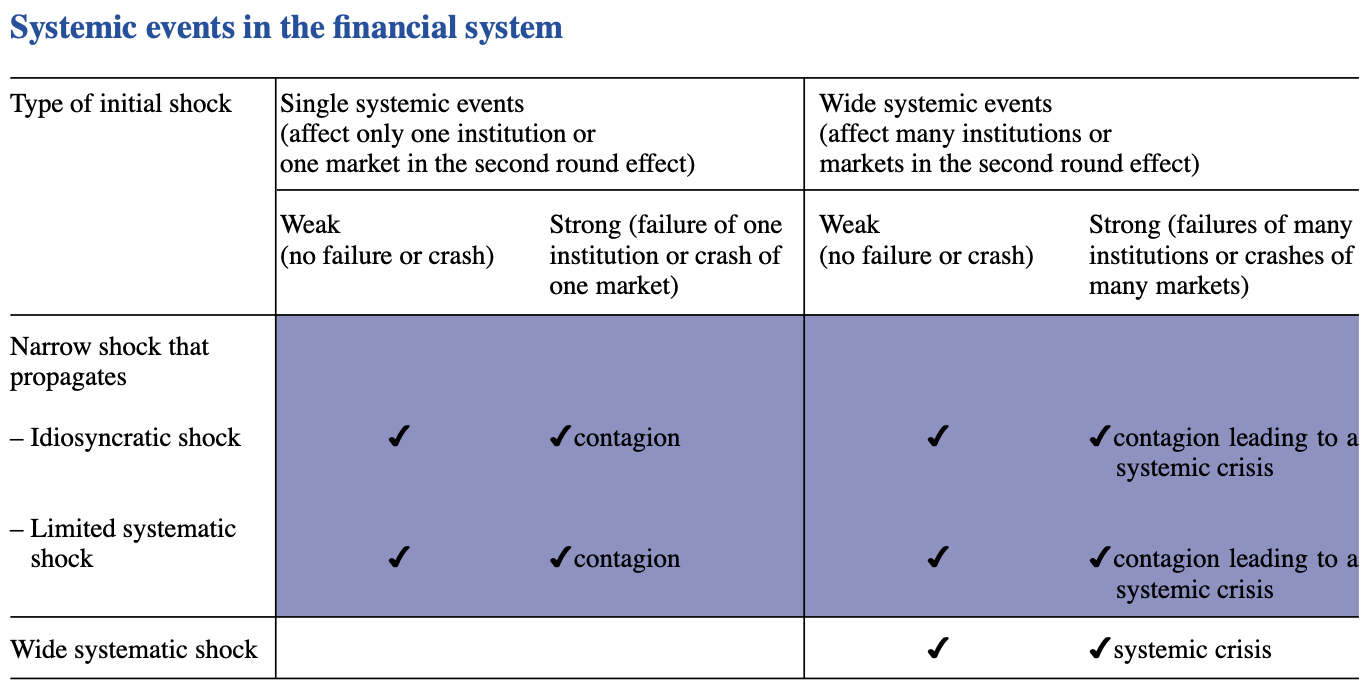
\includegraphics[width=1.0\linewidth]{images/systemic_events.png}
    \caption{\justifying \ding{51} signifie que la combinaison d’événements définie par la cellule constitue un événement systémique. La zone ombrée décrit les cas d’événements systémiques au sens restreint.
Les événements systémiques au sens large incluent également les cellules marquées \ding{51} dans la dernière ligne \citep{debandt2000systemic}.}
    \label{fig:systemic_vents}
\end{figure}

Sur la base de cette terminologie, une crise systémique (au sens restreint ou large) peut être définie comme un événement systémique qui affecte un nombre significatif d’institutions financières ou de marchés de manière forte, compromettant ainsi gravement le bon fonctionnement du système financier ou d’une partie essentielle de celui-ci. Le bon fonctionnement du système financier est ici entendu comme sa capacité à canaliser efficacement l’épargne vers les investissements productifs offrant les meilleurs rendements.\\

Par exemple, une crise financière systémique peut entraîner un rationnement extrême du crédit dans l’économie réelle, phénomène connu sous le nom de credit crunch. La distinction entre événements systémiques et crises systémiques est essentielle, car les mesures de gestion de crise varient en fonction de la nature du choc à l’origine du problème. Un choc idiosyncratique qui risque de provoquer une contagion nécessite une approche différente d’un choc systémique généralisé, qui engendre une déstabilisation simultanée de plusieurs segments du système financier. Cependant, dans la pratique, les situations de crise mêlent souvent chocs globaux et défaillances contagieuses. Par exemple, un ralentissement macroéconomique peut fragiliser des institutions financières, augmentant ainsi le risque de contagion des faillites individuelles. De même, un choc initial peut nécessiter l’effondrement de plusieurs institutions financières pour que la contagion se matérialise pleinement.

\subsubsection{Les symptômes observables du stress financier}

Les périodes de stress financier se manifestent par plusieurs symptômes observables qui traduisent les tensions et dysfonctionnements affectant les marchés financiers et le système bancaire. L’un des premiers signes d’un stress systémique est une volatilité accrue des prix des actifs. En temps normal, les fluctuations des prix des actions, obligations ou devises sont principalement dictées par les fondamentaux économiques et les anticipations des investisseurs. Cependant, en période de forte incertitude, les marchés deviennent plus instables, avec des variations de prix plus marquées et plus fréquentes. Cette volatilité reflète une augmentation des comportements spéculatifs et une réduction de la liquidité, rendant les transactions plus difficiles et amplifiant les mouvements de prix, parfois de manière excessive.\\

Un autre symptôme majeur du stress financier est une chute significative de la valorisation des actifs financiers. Lorsque les investisseurs anticipent une détérioration des conditions économiques ou des défaillances au sein du système financier, ils réévaluent leurs portefeuilles et procèdent à des ventes massives, ce qui entraîne un effondrement des prix des actifs. Ce phénomène a été particulièrement marqué lors de la crise financière de 2008, où la dévalorisation des actifs adossés aux crédits hypothécaires subprime a provoqué une spirale baissière, forçant de nombreuses institutions financières à enregistrer des pertes colossales. Cette perte de confiance généralisée se répercute sur l’ensemble du système financier, aggravant la crise et freinant la reprise économique.\\

Parallèlement, les primes de risque de défaut et de liquidité connaissent une forte augmentation en période de stress systémique. La prime de risque de défaut, qui reflète la probabilité qu’un emprunteur ne puisse pas honorer ses engagements financiers, tend à s’accroître lorsque les perspectives économiques se dégradent ou que la solvabilité des institutions financières est remise en question. Ce phénomène s’observe notamment à travers l’écartement des spreads obligataires, c’est-à-dire l’augmentation de l’écart entre les rendements des obligations d’État considérées comme sûres (telles que les Bunds allemands) et celles des pays ou entreprises perçus comme plus risqués. De même, la prime de liquidité augmente lorsque les investisseurs exigent une compensation plus élevée pour détenir des actifs difficiles à revendre en cas de besoin urgent de liquidités. Cela entraîne des distorsions dans la transmission des signaux de prix et exacerbe l’instabilité des marchés financiers.\\

Le stress systémique représente la manifestation concrète du risque systémique, dont les effets peuvent être dévastateurs pour l’économie si aucune mesure n’est prise pour le contenir. En distinguant les perspectives horizontale et verticale du risque systémique, il est possible d’adopter une approche plus complète pour analyser son impact et identifier les leviers d’intervention les plus efficaces. L’évaluation du risque systémique, notamment via des indicateurs comme le CISS, permet aux décideurs économiques d’anticiper les périodes de tension et d’adopter des politiques monétaires et macroprudentielles adaptées pour limiter la propagation des crises et préserver la stabilité financière.

\subsection{L'indicateur composite de stress systémique}

La stabilité du système financier repose sur l'équilibre des interactions entre les différents segments de marché. Cependant, cet équilibre est régulièrement menacé par des tensions systémiques, amplifiées par l'interconnexion croissante des marchés. Dans ce contexte, des outils d'analyse et de surveillance, tels que le \textit{Composite Indicator of Systemic Stress} (\textit{CISS}), se révèlent essentiels pour comprendre et anticiper les risques systémiques. Conçu pour capturer les signaux de stress financier à travers différents segments, cet indicateur composite intègre les spécificités des marchés actions, des changes, obligataire, des intermédiaires financiers et monétaires, tout en tenant compte de leurs interactions dynamiques.\\

Tout d'abord, il est introduit les fondements du \textit{CISS}, en expliquant son objectif principal : fournir une mesure agrégée du stress systémique tout en capturant les interdépendances entre les segments de marché. Puis, il est exploré son évolution depuis des outils plus sectoriels, tels que le \textit{SovCISS}, jusqu'à sa formulation actuelle, qui intègre des notions de corrélation dynamique entre marchés. Enfin, une attention particulière est portée à la formulation mathématique du \textit{CISS}, mettant en évidence les méthodologies de pondération et de calcul pour cet indicateur.

\subsubsection{Construction de l'indicateur composite de stress systémique}

Le \textit{CISS} est un outil central pour surveiller les tensions systémiques, en offrant une mesure agrégée du stress financier à travers différents segments de marché. Ce paragraphe explore d’abord sa présentation générale, en détaillant son rôle dans l’identification des risques systémiques. Ensuite, l’évolution de cet indicateur depuis le \textit{SovCISS} est discutée, mettant en lumière son passage d’un indicateur centré sur les obligations souveraines à une approche globale intégrant plusieurs segments financiers. Enfin, sa formulation mathématique est présentée, expliquant comment les sous-indicateurs sont normalisés, pondérés et agrégés pour refléter les interconnexions et les corrélations dynamiques entre les marchés. Cette structure vise à clarifier la construction et l’utilité de cet outil dans la gestion des risques financiers.

\subsubsection{Généralités}

Le \textit{CISS} est un outil clé pour la surveillance de la stabilité financière dans les économies modernes, notamment au sein de l'Union européenne. Conçu pour offrir une vue d'ensemble des tensions sur les marchés financiers, cet indicateur composite permet aux régulateurs, en particulier la BCE, d’évaluer le risque systémique en temps réel et d’adapter leurs politiques en conséquence. Le \textit{CISS} a pour objectif principal de détecter les périodes où les tensions financières se manifestent simultanément sur plusieurs segments des marchés, ce qui reflète un risque accru de perturbation de l’ensemble du système financier.\\

Le stress systémique désigne la situation où une instabilité financière locale ou sectorielle s'étend et affecte la stabilité de l'ensemble du système financier. Cette extension peut être provoquée par des interconnexions entre différents segments des marchés financiers, des comportements synchronisés des acteurs économiques, ou encore par des canaux de contagion tels que la liquidité ou la confiance des investisseurs. Lorsqu'une crise se généralise, elle peut perturber le fonctionnement normal des marchés, compromettant ainsi la fourniture de crédit, la stabilité des taux d'intérêt et des taux de change, ainsi que le bon déroulement des institutions financières. Cela peut, à terme, affecter gravement l'économie réelle en réduisant la croissance, en augmentant le chômage et en déstabilisant les secteurs productifs.\\

Dans ce contexte, le \textit{CISS} permet de capter les signaux de tensions financières à travers différents marchés, qu'il s'agisse du marché des actions, des obligations, du marché monétaire ou des changes. En captant ces signaux simultanément, le \textit{CISS} évalue si les tensions dans un segment particulier sont susceptibles de se propager aux autres segments, créant un effet de contagion susceptible de perturber l’ensemble du système financier.\\

Le \textit{CISS} se base sur l'idée que les marchés financiers ne fonctionnent pas en autarcie. Au contraire, ils sont fortement interconnectés, et une crise dans l'un d'eux peut rapidement se propager aux autres via divers canaux. Par exemple, une crise de liquidité sur le marché monétaire peut forcer les banques à vendre massivement leurs actifs financiers, y compris des actions ou des obligations, pour couvrir leurs besoins en liquidité, ce qui augmente la volatilité sur les marchés des actions et obligataires. De même, des fluctuations importantes sur le marché des changes, par exemple une dépréciation rapide d'une monnaie majeure comme l'euro ou le dollar, peuvent provoquer des ajustements significatifs dans les portefeuilles des investisseurs et des entreprises, avec des répercussions sur les marchés actions et obligations. \\

Ce dernier tient compte de ces interconnexions en agrégeant plusieurs sous-indicateurs de stress issus de différents segments du marché. Ces sous-indicateurs mesurent des aspects spécifiques du stress financier, comme la volatilité des prix des actions, les écarts de taux entre les obligations souveraines et les obligations d'entreprises, ou encore les tensions sur les taux interbancaires. En combinant ces informations dans un seul indicateur composite, le CISS offre une mesure globale du risque systémique, tout en accordant une attention particulière aux périodes où les tensions apparaissent simultanément sur plusieurs segments des marchés.\\

Aussi, des caractéristiques majeures de l'indicateur sont qu'il accorde une importance particulière aux corrélations dynamiques entre les différents segments du marché. En période normale, les tensions sur un marché peuvent rester localisées et ne pas se propager aux autres segments. Cependant, en période de crise, ces corrélations tendent à augmenter, ce qui signifie que les chocs dans un segment particulier, comme le marché des actions, ont plus de chances de se transmettre aux autres segments, comme le marché des changes ou le marché monétaire. Le CISS capture cette augmentation des corrélations en attribuant un poids plus important aux périodes où plusieurs marchés sont simultanément sous pression. Ainsi, plus les tensions sont corrélées entre les marchés, plus le CISS augmentera, signalant un risque systémique accru. Cette approche permet de différencier les périodes de stress localisé, qui peuvent ne pas représenter un risque pour l'ensemble du système financier, des périodes de stress systémique, où la contagion entre les segments du marché est plus probable. Cela aide les régulateurs à concentrer leurs efforts sur les périodes où les risques systémiques sont les plus élevés et à ajuster leur politique monétaire ou macroprudentielle en conséquence.\\

L'une des raisons pour lesquelles le CISS est particulièrement précieux pour les régulateurs comme la BCE est qu'il permet de détecter les risques avant qu'ils ne deviennent visibles à travers d'autres indicateurs économiques. En surveillant en permanence l'état des différents segments des marchés financiers, le CISS permet aux régulateurs de réagir de manière proactive aux signes de stress systémique. Cela est particulièrement important dans les économies modernes, où les marchés financiers jouent un rôle essentiel dans l'allocation des ressources et le financement de l'activité économique. De plus, le CISS est un outil précieux pour la politique macroprudentielle, qui vise à prévenir les crises financières avant qu'elles ne se matérialisent. En identifiant les périodes de risque systémique élevé, les régulateurs peuvent prendre des mesures pour renforcer la résilience du système financier, pour illustrer en augmentant les exigences de fonds propres des banques, en imposant des limites sur l'exposition aux risques ou en renforçant les liquidités des institutions financières. L'objectif est de prévenir la contagion des crises financières, de sorte que même en cas de choc sur un segment particulier du marché, le reste du système financier reste suffisamment solide pour absorber ce choc sans s'effondrer.\\

Ainsi, l'utilité de l'indicateur ne se limite pas à la surveillance des marchés financiers. Il joue également un rôle crucial dans la protection de l'économie réelle contre les perturbations financières. Lorsqu'une crise financière devient systémique, elle affecte non seulement les marchés financiers, mais aussi l'économie dans son ensemble. Les entreprises trouvent plus difficile de se financer, les ménages réduisent leurs dépenses en raison des incertitudes économiques, et les banques deviennent plus réticentes à prêter, ce qui aggrave encore la contraction de l'activité économique. En aidant à prévenir les crises systémiques, le CISS contribue indirectement à la stabilité de l'économie réelle, en assurant que les marchés financiers continuent de fonctionner de manière fluide, même en période de tension.\\ 

Après ces généralités il convient de comprendre l'histoire de l'indicateur avant d'aborder son développement.

\subsubsection{Du SovCISS au CISS}

Avant l'introduction du \textit{CISS}, la BCE et d'autres institutions financières utilisaient un autre indicateur appelé \textit{SovCISS} (Sovereign Composite Indicator of Systemic Stress), conçu spécifiquement pour mesurer le stress systémique lié aux marchés des obligations souveraines. Le \textit{SovCISS} a été développé à une époque où les crises de dette souveraine, en particulier celles qui ont frappé la zone euro entre 2010 et 2012, étaient au centre des préoccupations des régulateurs. Cet indice visait à capter les tensions sur les marchés des obligations d'État, en tenant compte des spreads entre les obligations souveraines des pays membres de la zone euro et les obligations dites « sans risque », comme celles de l'Allemagne. En période de crise, les écarts entre les taux d’intérêt des obligations d’États comme ceux de la Grèce ou de l’Italie par rapport à l’Allemagne augmentaient de manière significative, signalant une perte de confiance des investisseurs dans la capacité des gouvernements à honorer leurs dettes.\\

Cependant, bien que le \textit{SovCISS} ait été un outil utile pour comprendre les dynamiques de la crise de la dette souveraine, il est devenu évident qu'un indice uniquement centré sur les obligations souveraines était insuffisant pour mesurer les risques systémiques globaux. Les crises financières récentes, comme celle des subprimes de 2007-2008, ont montré que les crises systémiques ne se limitaient pas à un seul segment, mais résultaient d'une propagation rapide des tensions entre les différents marchés financiers. Ainsi, la BCE a reconnu la nécessité de développer un indicateur plus global, capable de capter les interactions et les tensions simultanées à travers plusieurs segments financiers, tels que les marchés des changes, des actions, des obligations privées, et des banques. C’est dans ce contexte que le \textit{CISS} a été introduit.\\

Le \textit{CISS} surpasse le \textit{SovCISS} en ce qu’il intègre une mesure de la corrélation dynamique entre les segments du marché. Alors que le \textit{SovCISS} se concentrait principalement sur les tensions dans le secteur des obligations souveraines, le \textit{CISS} capte les tensions qui se propagent à travers tous les segments, offrant ainsi une vision plus complète du stress systémique. Il permet non seulement de surveiller les tensions dans chaque segment, mais aussi d’évaluer comment ces tensions interagissent et s’amplifient entre eux. Le passage du \textit{SovCISS} au \textit{CISS} est une évolution dans la manière dont les régulateurs financiers, et en particulier la BCE, appréhendent les crises systémiques : d’une approche sectorielle centrée sur les obligations souveraines à une approche globale qui prend en compte l'ensemble des segments du système financier et leurs interconnexions.

\subsubsection{Le développement du \textit{CISS}}

Les crises financières récentes, notamment la crise des subprimes de 2007-2008, ont montré à quel point les chocs financiers pouvaient rapidement se propager à travers différents segments du système financier, déclenchant ainsi des crises systémiques d’une ampleur sans précédent. Avant la création du \textit{CISS}, les outils de surveillance disponibles, bien qu'utiles pour comprendre certains aspects des marchés financiers, étaient trop fragmentés et ne permettaient pas de saisir pleinement l'ampleur ni la portée des risques systémiques. Ces outils étaient principalement axés sur des indicateurs spécifiques à chaque segment, tels que les taux interbancaires, les spreads obligataires ou la volatilité des marchés actions, sans intégrer de manière adéquate les interconnexions entre les différents segments. Cela créait une lacune dans la surveillance globale des risques financiers, notamment en ce qui concerne l’anticipation de crises systémiques.\\

L'indicateur répond à ce besoin en fournissant une mesure agrégée du stress systémique, capable de capturer les tensions qui surviennent simultanément dans plusieurs secteurs du système financier. Ce cadre analytique plus intégré s’est révélé essentiel après la crise des subprimes, une période où les indicateurs traditionnels avaient échoué à identifier les signes avant-coureurs d’une crise mondiale. La crise de 2007-2008 a particulièrement mis en lumière les insuffisances des indicateurs sectoriels pour surveiller et anticiper les risques financiers. Les outils utilisés à cette époque étaient trop compartimentés, focalisés sur des segments isolés des marchés, ce qui empêchait de saisir l'ampleur des interconnexions et de l’effet de contagion qui allait finalement provoquer un effondrement général du système financier. Le CISS a été conçu pour combler cette lacune en offrant une vue d’ensemble des risques systémiques en agrégeant les tensions dans les principaux segments financiers : le secteur bancaire, les marchés obligataires, les marchés des actions, les marchés des changes, et d’autres segments financiers clés.\\

Son développement repose sur des concepts tirés de la théorie des portefeuilles, développée par Harry Markowitz dans les années 1950. Cette théorie met en évidence le rôle crucial de la diversification pour optimiser un portefeuille d’actifs en termes de rentabilité maximale et de risque minimal. De la même manière, cet indicateur applique ce principe à la gestion du risque systémique en combinant plusieurs segments du système financier tout en tenant compte des corrélations temporelles entre eux. Chaque segment est susceptible de subir des chocs qui peuvent se propager aux autres segments par le biais de multiples canaux de transmission. L’indicateur reflète donc non seulement les tensions dans chaque segment, mais aussi la manière dont ces tensions interagissent et s’amplifient à travers les interconnexions systémiques. C'est donc un outil global particulièrement pertinent pour mesurer le risque systémique à un instant donné.\\

En outre, cet indicateur permet de surveiller en temps réel les tensions qui se manifestent dans les différents segments du système financier. Cela en fait une métrique particulièrement précieuse pour les banques centrales et les autorités financières, car il leur offre la possibilité de détecter les signes précoces de crises potentielles et de mettre en place des mesures préventives pour stabiliser le système. En identifiant les périodes de stress simultané sur plusieurs segments, il permet d’anticiper les crises avant qu’elles ne deviennent trop graves et d’intervenir de manière proactive. Il constitue également un outil d’analyse rétrospective, permettant d’examiner les crises passées et d’évaluer les niveaux de stress atteints durant ces périodes critiques. Il est donc possible d’établir des comparaisons entre différentes crises financières et d’en analyser les dynamiques propres, facilitant ainsi l’évaluation des politiques et des mesures mises en place pour répondre à ces crises.\\

Par exemple, en comparant les niveaux atteints durant la crise des subprimes à ceux observés pendant la crise de la dette souveraine en Europe, il est possible d’évaluer l’efficacité des réponses monétaires et fiscales appliquées dans chacun de ces cas. Ce type d’analyse comparative permet également de tirer des enseignements utiles pour la gestion des futures crises. Une analyse approfondie des dynamiques de chaque crise aide les régulateurs à mieux comprendre les mécanismes de propagation des tensions financières et à ajuster leurs outils en conséquence.\\

Cet indicateur agit également comme un outil de rétroaction particulièrement utile pour les décideurs politiques et monétaires. Après une intervention de la banque centrale, une baisse significative de l’indicateur signalerait que les mesures prises ont effectivement contribué à réduire les tensions dans le système financier. Cette capacité d’évaluer les réponses politiques et monétaires en temps réel confère à cet outil un rôle unique dans la gestion des crises financières. Contrairement aux indicateurs traditionnels qui ne captent que des aspects isolés du marché, il permet une vision plus holistique des risques, facilitant ainsi des réponses politiques plus efficaces et mieux ciblées.\\

Il est décomposé en cinq indices principaux, chacun représentant un segment majeur du marché financier, tels que le secteur bancaire, les marchés obligataires, les marchés des actions, les marchés des changes et les autres segments financiers pertinents. Chacun de ces indices est ensuite subdivisé en sous-indices qui capturent des aspects spécifiques de leurs segments respectifs, comme la volatilité des actions, les spreads des obligations souveraines ou les tensions sur les taux interbancaires. Cette structure hiérarchisée permet à l’outil d’offrir une vision à la fois large et détaillée des tensions financières, tout en tenant compte des interdépendances entre les segments. L’agrégation de ces indices, en tenant compte des corrélations entre eux, permet de générer un indicateur composite qui mesure le niveau global de risque systémique auquel est confronté le système financier.\\

L’innovation apportée par cet indicateur réside donc dans sa capacité à offrir une mesure intégrée et dynamique des risques financiers. Contrairement aux approches traditionnelles, qui se concentrent sur l’intensité des tensions dans des segments spécifiques, il prend en compte la propagation et la diffusion de ces tensions à travers l’ensemble du système financier. Cela permet aux régulateurs de mieux comprendre la manière dont les chocs financiers se propagent entre les différents segments et d’anticiper l’apparition de crises systémiques. En intégrant à la fois l’intensité des tensions et leur diffusion à travers le système, cet outil devient central pour la gestion et l’anticipation des crises financières.

%Graphique 

\subsubsection{Formulation mathématique du \textit{CISS}}

Le \textit{CISS} repose sur cinq indices, chacun étant lui-même subdivisé en plusieurs sous-indices. Ces indices principaux sont pondérés en fonction de leur importance relative, avec des coefficients spécifiques attribués à chaque sous-indice, ce qui permet d'obtenir une mesure globale du risque systémique. Les poids attribués aux indices déterminent leur influence sur le calcul final du \textit{CISS}. La construction mathématique suivante est reprise de \citep{hollo2012ciss}.

\begin{enumerate}
    \item  30\% pour le marché intermédiaire
    \item 25\% pour le marché des actions 
    \item 15\% pour le marché obligataire 
    \item 15\% pour le marché monétaire
    \item 15\% pour le marché des changes
\end{enumerate}

Pour chaque segment de marché, trois indicateurs de stress financier sont sélectionnés, notés \( x_{t,i,j} \). Soit un ensemble de valeurs observées \( x_1, x_2, \dots, x_n \) pour un indicateur spécifique. On ordonne ces valeurs de telle sorte que \( x_{[1]} \leq x_{[2]} \leq \dots \leq x_{[n]} \), où \( x_{[r]} \) représente le \( r \)-ième ordre de valeur. De plus,

\begin{itemize}
    \item \( t \) représente le temps,
    \item \( i \) indique le segment de marché (\( i = 1, 2, 3, 4, 5 \) pour les marchés monétaires, obligations, actions, intermédiaires financiers, et changes),
    \item \( j \) correspond à chaque indicateur spécifique dans le segment (\( j = 1, 2, 3 \)).
\end{itemize}

Ces indicateurs sont normalisés en utilisant leur fonction de distribution cumulative empirique \( F(x_{t,i,j}) \), ce qui donne le score normalisé :
\begin{equation}
z_{t,i,j} = F(x_{t,i,j}) = \frac{r}{n}
\end{equation}
où \( r \) est le rang de \( x_{t,i,j} \) dans un ensemble de \( n \) observations, ordonnées de manière croissante. La transformation est mise à jour de manière récursive pour chaque nouvelle observation \( T \) :
\begin{equation}
z_{T,i,j} = F_{T}(x_{T,i,j}) = \frac{r}{T}
\end{equation}

Par la suite, pour chaque segment de marché \( i \), un sous-indice \( s_{t,i} \) est construit en prenant la moyenne arithmétique des trois indicateurs normalisés :
\begin{equation}
s_{t,i} = \frac{1}{3} \sum_{j=1}^{3} z_{t,i,j}
\end{equation}

Enfin, les cinq sous-indices sont agrégés dans un indicateur composite \( CISS_t \) en utilisant des poids \( w_i \) représentant leur importance pour l'activité économique réelle. Le vecteur de poids est \( w = [0.15, 0.15, 0.25, 0.30, 0.15] \). Le CISS est calculé en tenant compte des corrélations dynamiques entre les segments :
\begin{equation}
CISS_t = \left( w \circ s_t \right)^T C_t \left( w \circ s_t \right) = \sum_{i=1}^{5} \sum_{j=1}^{5} w_i w_j s_{t,i} s_{t,j} \rho_{t,ij}
\end{equation}
où \( w \circ s_t \) représente le produit de Hadamard (élément par élément) entre le vecteur de poids \( w \) et le vecteur des sous-indices \( s_t = [s_{t,1}, s_{t,2}, s_{t,3}, s_{t,4}, s_{t,5}] \), et \( C_t \) est la matrice de corrélation des sous-indices.\\

Aussi, la matrice de corrélation \( C_t \) est une matrice symétrique \( 5 \times 5 \), où chaque élément \( \rho_{t,ij} \) représente la corrélation entre les sous-indices \( s_{t,i} \) et \( s_{t,j} \) :

\begin{equation}
C_t = \begin{bmatrix}
1 & \rho_{t,12} & \rho_{t,13} & \rho_{t,14} & \rho_{t,15} \\
\rho_{t,12} & 1 & \rho_{t,23} & \rho_{t,24} & \rho_{t,25} \\
\rho_{t,13} & \rho_{t,23} & 1 & \rho_{t,34} & \rho_{t,35} \\
\rho_{t,14} & \rho_{t,24} & \rho_{t,34} & 1 & \rho_{t,45} \\
\rho_{t,15} & \rho_{t,25} & \rho_{t,35} & \rho_{t,45} & 1 \\
\end{bmatrix}
\end{equation}

Les éléments de la matrice \( C_t \) sont calculés en fonction des covariances \( \sigma_{t,ij} \) et des écarts-types des sous-indices respectifs \( \sigma_{t,i} \) et \( \sigma_{t,j} \) :

\begin{equation}
\rho_{t,ij} = \frac{\sigma_{t,ij}}{\sqrt{\sigma_{t,i}^2 \cdot \sigma_{t,j}^2}}
\end{equation}

Les covariances et variances sont calculées de manière récursive avec des moyennes mobiles exponentielles :

\begin{equation}
\sigma_{t,i}^2 = \lambda \sigma_{t-1,i}^2 + (1 - \lambda) \tilde{s}_{t,i}^2
\end{equation}

\begin{equation}
\sigma_{t,ij} = \lambda \sigma_{t-1,ij} + (1 - \lambda) \tilde{s}_{t,i} \tilde{s}_{t,j}
\end{equation}

où \( \lambda \) est un paramètre de lissage, typiquement autour de 0.93 \citep{hollo2012ciss}, et \( \tilde{s}_{t,i} \) est le sous-indice centré autour de sa moyenne historique.\\

Le stress systémique constitue une menace majeure pour la stabilité du système financier européen, amplifiée par les interconnexions croissantes entre les segments de marché et les institutions financières. Sa compréhension nécessite une analyse fine des dynamiques de contagion, des niveaux d'intensité des événements systémiques, ainsi que des symptômes observables lors des épisodes de crise. Dans ce contexte, l’indicateur composite de stress systémique (\textit{CISS}) s’impose comme un outil de surveillance particulièrement pertinent. Il permet ainsi d’anticiper les phases critiques et d’ajuster les réponses politiques en conséquence. Toutefois, la surveillance des risques systémiques ne saurait se limiter à une lecture technique des indicateurs. Elle nécessite également une réflexion sur les leviers d’action mobilisables pour limiter la propagation des crises. Parmi ces leviers, la politique monétaire — et en particulier la forward guidance — joue un rôle croissant dans la gestion des anticipations et des tensions sur les marchés financiers.\\

C’est pourquoi il est ensuite proposé d’examiner les interactions entre la forward guidance et le stress systémique, en analysant dans quelle mesure une communication stratégique efficace de la banque centrale peut contribuer à prévenir, amortir ou au contraire amplifier les épisodes de turbulence financière.

\section{Stress systémique et forward guidance}

L’analyse du lien entre la forward guidance et le stress systémique constitue un champ d’étude encore relativement peu exploré, malgré l’importance croissante de ces deux concepts dans la politique monétaire moderne. La forward guidance est largement reconnue comme un instrument central permettant aux banques centrales d’influencer les anticipations des agents économiques et de renforcer la transmission de la politique monétaire. Parallèlement, le stress systémique, qui résulte de perturbations majeures affectant l’ensemble du système financier, représente une préoccupation majeure pour les autorités monétaires et macroprudentielles. Toutefois, la manière dont la forward guidance interagit avec le stress systémique demeure peu étudiée dans la littérature. Alors que de nombreuses recherches ont porté sur le rôle des taux d’intérêt et des mesures non conventionnelles dans la stabilité financière, peu d’études se sont focalisées sur l’impact spécifique des stratégies de communication des banques centrales dans la prévention ou l’amplification des tensions financières. Dans un contexte où la BCE et d’autres institutions monétaires s’appuient de plus en plus sur la forward guidance pour stabiliser les marchés et orienter les anticipations, il apparaît essentiel de comprendre dans quelle mesure cet outil peut influencer le niveau de stress systémique. La forward guidance peut-elle réellement réduire les tensions financières en apportant de la visibilité aux investisseurs et aux intermédiaires financiers ? Ou, au contraire, peut-elle accroître le stress systémique en cas de perte de crédibilité ou de mauvaise interprétation par les marchés ? Ce paragraphe propose d’analyser ces questions en approfondissant les interactions entre ces deux dynamiques fondamentales.L’examen de cette relation se fera en trois étapes. Tout d’abord, l’impact de la forward guidance sur le stress systémique fera l'objet d'une étude, en mettant en lumière les mécanismes par lesquels cet outil peut contribuer à atténuer ou, au contraire, à exacerber les tensions sur les marchés financiers. Il analysera notamment comment une forward guidance claire et crédible peut jouer un rôle stabilisateur en période de crise, en réduisant l’incertitude et en limitant la volatilité des marchés. Toutefois, les risques liés à une mauvaise gestion de la forward guidance seront également explorés, notamment en ce qui concerne la perte de crédibilité des banques centrales et les distorsions de marché qu’une politique mal calibrée peut engendrer.Ensuite, l’interaction entre la forward guidance et la régulation macroprudentielle sera abordée. Il sera examiné dans quelle mesure la forward guidance peut compléter ou entrer en conflit avec les mesures de stabilité financière mises en place par les autorités macroprudentielles. La nécessité d’une coordination entre ces deux approches est mise en évidence, afin d’éviter que les effets de la forward guidance ne compromettent l’efficacité des mesures prudentielles, et inversement. Enfin, une attention particulière portera sur les limites et les défis d’une coordination insuffisante entre la politique monétaire et la régulation macroprudentielle. Cela montrera comment une communication mal alignée avec les mesures macroprudentielles peut générer de l’incertitude et accroître le stress systémique, notamment lorsque les signaux envoyés aux marchés financiers deviennent contradictoires. À travers cette analyse, sont ainsi mises en évidence les implications de la forward guidance pour la stabilité du système financier et les précautions à prendre pour éviter qu’elle ne devienne une source supplémentaire de stress systémique

\subsection{Impact de la forward guidance sur le stress systémique}

La forward guidance, en influençant les anticipations des agents économiques, peut aussi jouer un rôle dans la réduction ou l’amplification du stress systémique au sein du système financier. Le stress systémique, souvent provoquées par des crises de liquidité, des faillites bancaires ou des pertes de confiance généralisées dans le système financier. Dans ce contexte, la capacité des banques centrales à ancrer efficacement les anticipations via la forward guidance peut contribuer à limiter les risques de propagation des crises.

\subsubsection{La forward guidance comme outil de réduction du stress systémique}

Une forward guidance claire, crédible et bien communiquée peut jouer un rôle stabilisateur en période de stress systémique. L’un des principaux canaux par lesquels elle agit est la réduction de l’incertitude macroéconomique et financière. En fournissant aux agents économiques des indications précises sur l’orientation future des taux d’intérêt et des conditions monétaires, la forward guidance permet d’ancrer les anticipations et de limiter la volatilité excessive des marchés \citep{woodford2012}).\\

Par exemple, lors de la crise des dettes souveraines en 2012, la déclaration de Mario Draghi affirmant que la BCE ferait "whatever it takes" pour préserver l’euro a eu un effet immédiat de réduction du stress systémique. Cette simple communication a permis de restaurer la confiance des investisseurs et d'éviter une fragmentation accrue des marchés obligataires de la zone euro \citep{Acharya2015}. La forward guidance peut donc jouer un rôle similaire à celui d’un pare-feu psychologique, en signalant aux marchés que la banque centrale est prête à intervenir pour stabiliser le système financier.\\

De plus, en périodes de crises financières, la forward guidance peut atténuer le risque de contagion en fixant un cap clair sur l’évolution future des conditions monétaires. Une politique monétaire imprévisible ou perçue comme hésitante peut engendrer des comportements procycliques, où les investisseurs réduisent leur exposition au risque de manière excessive, aggravant ainsi la crise. En maintenant des engagements crédibles sur la trajectoire des taux d’intérêt, la forward guidance permet d’éviter des ventes massives d’actifs et un durcissement excessif des conditions financières \citep{swanson2021}.

\subsubsection{Risques et effets indésirables de la forward guidance sur le stress systémique}

Si la forward guidance peut être un instrument stabilisateur, elle présente aussi des risques potentiels qui peuvent, sous certaines conditions, aggraver le stress systémique. L’un des principaux dangers réside dans une perte de crédibilité de la banque centrale. Lorsque les marchés perçoivent que la forward guidance n’est pas suivie d’actions cohérentes, cela peut créer un climat d’incertitude accru, qui amplifie la volatilité des marchés financiers.\\

Un exemple marquant de ce phénomène est le "Taper Tantrum" de 2013, où l’annonce prématurée d’un ralentissement des achats d’actifs par la Réserve fédérale américaine (Fed) a provoqué une flambée des taux d’intérêt à long terme et un effondrement des marchés émergents. Cette réaction excessive s’explique par un changement soudain de forward guidance, mal anticipé par les investisseurs \citep{gürkaynak2015}. Cet épisode illustre comment une mauvaise gestion des attentes peut engendrer une crise de liquidité et de confiance, exacerbant ainsi le stress systémique.\\

Un autre problème réside dans le risque de distorsions financières et de prise de risque excessive. Une forward guidance trop accommodante, en signalant un maintien prolongé des taux bas, peut inciter les investisseurs à rechercher des rendements plus élevés en prenant des risques excessifs. Ce phénomène, connu sous le nom de "search for yield", peut gonfler des bulles financières et fragiliser le système bancaire en période de resserrement monétaire. Par exemple, la période prolongée de taux bas après la crise financière de 2008 a favorisé une accumulation de dettes privées et une montée des valorisations boursières, augmentant la vulnérabilité du système financier en cas de choc externe.

\newpage

Le stress systémique résulte souvent d’interactions entre déséquilibres macroéconomiques, comportements. Alors, il est essentiel d’examiner comment la forward guidance peut s’articuler avec d’autres outils de gestion du risque systémique, notamment la régulation macroprudentielle.

\subsection{Interactions entre forward guidance et régulation macroprudentielle dans la gestion du stress systémique}

Dans ce paragraphe il est montré l’interaction entre la forward guidance et la régulation macroprudentielle dans la gestion du stress systémique. La complémentarité entre ces deux outils permet de stabiliser les anticipations des marchés et de limiter les déséquilibres financiers liés à des politiques monétaires accommodantes prolongées.  Cependant, en l’absence de coopération étroite, des conflits d’objectifs peuvent apparaître, augmentant l’incertitude et la volatilité des marchés. L’étude de ces interactions est donc essentielle pour affiner la communication des banques centrales et renforcer la stabilité financière.

\subsubsection{La complémentarité entre forward guidance et régulation macroprudentielle}

La forward guidance, en tant qu'outil central de communication des banques centrales, joue un rôle déterminant en influençant les anticipations des marchés financiers. Son objectif est de clarifier les intentions futures en matière de politique monétaire afin d’orienter les attentes des acteurs économiques vers des scénarios souhaités par les autorités monétaires. Cependant, cette stratégie doit nécessairement interagir de manière étroite avec la régulation macroprudentielle, dont la finalité principale est de limiter l'accumulation de risques systémiques susceptibles de déstabiliser l'économie globale. Selon les travaux pionniers de \citep{BorioZhu2012}, la coordination étroite entre la forward guidance et les instruments de régulation macroprudentielle permet une gestion plus efficace du stress systémique. En effet, une politique macroprudentielle rigoureuse peut renforcer la crédibilité et l'efficacité de la forward guidance en rassurant les acteurs économiques sur le fait que les risques financiers demeureront maîtrisés, même en situation prolongée de taux d'intérêt très bas. \citep{FilardoHofmann2014} soulignent à cet égard que la confiance dans la stabilité financière rend les anticipations des acteurs économiques plus robustes, facilitant ainsi l'atteinte des objectifs de la politique monétaire. \citep{GalatiMoessner2018} approfondissent cette analyse en montrant que la combinaison stratégique de la forward guidance avec des politiques macroprudentielles permet une stabilisation accrue des anticipations des marchés financiers. Cette combinaison réduit significativement les risques de formation de bulles spéculatives, lesquelles constituent une menace importante pour la stabilité financière à long terme. Ainsi, en évitant les excès d'optimisme ou de pessimisme sur les marchés, cette coordination améliore considérablement l'efficacité globale de la politique monétaire. Par ailleurs, \citep{Smets2014} insiste sur l'importance d'une coordination proactive entre ces deux politiques. Une telle approche anticipative permet aux banques centrales et aux autorités macroprudentielles d’ajuster de manière optimale les anticipations des agents économiques, minimisant ainsi l'incertitude et la volatilité financière qui peuvent surgir lors de périodes prolongées de politique monétaire accommodante. En agissant conjointement, les autorités monétaires et prudentielles sont ainsi mieux placées pour gérer efficacement les périodes complexes où l’équilibre économique est particulièrement sensible aux variations d’anticipations des marchés.

\subsubsection{Risques et limites d’une coordination insuffisante}

Cependant, l’absence d’une coordination adéquate entre forward guidance et régulation macroprudentielle peut générer des conflits et réduire significativement l’efficacité des politiques mises en œuvre. \citep{farhi2016} soulignent explicitement que, sans une coopération étroite, les objectifs de stabilisation financière peuvent entrer en conflit direct avec ceux de la politique monétaire, particulièrement lorsque des taux d'intérêt bas prolongés incitent les acteurs financiers à adopter des comportements de prise de risque excessifs. Ce phénomène peut alors conduire à une accumulation dangereuse de déséquilibres financiers, menaçant la stabilité du système économique. \citep{claessens2013} préconisent ainsi une approche intégrée impliquant un échange actif et continu d'informations entre les banques centrales et les autorités macroprudentielles. Selon eux, une telle coordination permet d’éviter efficacement les effets secondaires indésirables des politiques individuelles. Par exemple, elle réduit les risques de formation de bulles spéculatives ou de surchauffe des marchés, tout en limitant les comportements risqués encouragés par des conditions monétaires accommodantes prolongées. Par ailleurs, \citep{rey2015} met en garde contre les conséquences potentiellement graves d’une coordination insuffisante. Des politiques contradictoires ou mal coordonnées peuvent en effet générer des signaux confus pour les marchés financiers, augmentant ainsi l’incertitude et aggravant le stress systémique. Cette confusion peut conduire à une volatilité accrue et à une instabilité financière qui, à son tour, nuit gravement à la réalisation des objectifs économiques globaux. Plus récemment, \citep{linta2024} met en évidence l'importance de la crédibilité dans l'efficacité de la forward guidance, soulignant que cette crédibilité dépend en grande partie d'une des votes en conseil des gouverneurs.\\

Dans ce cadre, étudier spécifiquement l'impact de la forward guidance sur le stress systémique est important pour les régulateurs. Une meilleure compréhension de cet impact permettrait aux décideurs publics d'affiner leur communication et de calibrer précisément leurs messages afin de réduire l’incertitude sur les marchés financiers, limitant ainsi les risques d’instabilité et de crises systémiques potentielles. Également, en analysant précisément les mécanismes par lesquels la forward guidance influence les anticipations des acteurs économiques, les régulateurs pourraient mieux anticiper et contrôler les comportements de prise de risque excessifs qui accompagnent souvent les périodes prolongées de politique monétaire accommodante. Enfin, une recherche approfondie sur ce sujet pourrait également fournir des orientations précieuses quant à l’articulation optimale entre la forward guidance et les mesures macroprudentielles, permettant ainsi aux régulateurs de mieux coordonner ces politiques et d’améliorer globalement l’efficacité de leur gestion du risque systémique.

\newpage

Dans ce chapitre, l'analyse du lien entre stress systémique et forward guidance met en évidence le rôle central que joue la communication des banques centrales dans la stabilité financière. En influençant les anticipations des agents économiques, la forward guidance peut à la fois réduire l’incertitude et limiter la volatilité des marchés, contribuant ainsi à la prévention des crises financières. Cependant, son efficacité repose sur deux piliers fondamentaux : la crédibilité des engagements des banques centrales et la cohérence des signaux envoyés aux marchés. Une forward guidance bien calibrée peut atténuer les tensions financières en ancrant les anticipations et en stabilisant les conditions monétaires, comme l’a illustré la réponse de la BCE lors de la crise des dettes souveraines.Toutefois, des risques demeurent. Une communication inadaptée ou une perte de crédibilité peuvent accentuer le stress systémique en créant de l’incertitude et en amplifiant les mouvements de marché. De plus, l’effet de la forward guidance sur les comportements d’investissement peut, en période prolongée de taux bas, favoriser des prises de risque excessives et la formation de bulles financières, augmentant ainsi la vulnérabilité du système financier.\\

L’interaction entre la forward guidance et la régulation macroprudentielle apparaît dès lors comme un levier essentiel pour assurer une gestion efficace du stress systémique. Une coordination renforcée entre ces deux outils permettrait de stabiliser les anticipations tout en limitant l’accumulation des déséquilibres financiers. À l’inverse, une absence de coordination ou des signaux contradictoires entre politique monétaire et régulation macroprudentielle risquent de fragiliser davantage le système financier, compromettant ainsi l’objectif de stabilité macroéconomique. Ainsi, la compréhension approfondie des interactions entre stress systémique et forward guidance constitue un enjeu majeur pour les banques centrales et les régulateurs financiers. Face à des crises financières de plus en plus interconnectées, il apparaît essentiel d’affiner les outils de communication monétaire et d’assurer une complémentarité efficace avec les mesures macroprudentielles. L’analyse du stress systémique et de ses déterminants, notamment à travers des indicateurs comme le \textit{CISS}, doit ainsi s’intégrer pleinement dans l’élaboration des stratégies monétaires et prudentielles. En définitive, une forward guidance efficace et cohérente avec les objectifs de stabilité financière représente un instrument puissant pour prévenir les crises et renforcer la résilience du système financier européen.\\

Afin d'étudier correctement le rôle de la forward guidance dans la dynamique du stress systémique, il est indispensable de modéliser rigoureusement ses mécanismes de transmission et ses effets différés sur les marchés financiers. En effet, les annonces de politique monétaire ne produisent pas des réactions instantanées, linéaires ou uniformes : leur impact dépend fortement des anticipations, des conditions de marché préexistantes, et peut se manifester de manière progressive ou différenciée selon les canaux de transmission. Le caractère temporel, non linéaire et parfois latent de ces réactions économiques appelle à mobiliser des outils capables de capturer des dépendances de long terme, de modéliser des régimes dynamiques sous-jacents. Le second chapitre se consacre ainsi à l’exploration des architectures neuronales avancées les plus pertinentes pour cette tâche afin de mémoriser et représenter les signaux de politique monétaire, dans le but de mesurer leur effet sur les dynamiques de stress systémique.